%
% $Id$
% A template to build SAND reports. See the examples for more details and
% formatting suggestions. A command reference is available at
% http://www.cs.sandia.gov/~rolf/SANDreport
%
\documentclass[pdf,12pt,relaxed]{SANDreport}


% Packages.
\usepackage{amsmath,amssymb,amsthm,bm}
\usepackage{enumerate}
\usepackage{verbatim}
\usepackage{pgf}
\usepackage{pgfpages}
\usepackage{pgfpages}
\usepackage{tikz}
%\usetikzlibrary{arrows,backgrounds}
\usepgflibrary{shapes}
\usepackage[bf]{caption} % caption v1.x
\usepackage{url}
\usepackage{hyperref}
\usepackage{amsfonts}
\usepackage{latexsym}
\usepackage{amssymb}
\usepackage{graphicx}

%\input{latexdefs}

\newtheorem{defin}{Definition}
\newtheorem{exam}{Example}

% ---------------------------------------------------------------------------- %
% Set the title, author, and date
%
    \title{Domain model and implementation of cell topology data}
    \author{Pavel Bochev\\
    		Applied Mathematics and Application Dept. 1414, MS-1320\\
                Sandia National Laboratories\\
                Albuquerque, NM 87185-1320\\
                pbboche@sandia.gov
                \\[0.2in]
             	Harold C. Edwards \\ 
             	Computational Thermal and Fluid Mechanics Dept. 1542,  MS-???? \\
                Sandia National Laboratories\\
                Albuquerque, NM 87185-????\\
             	hcedwar@sandia.gov \\[0.2in]
		Roger Pawlowski\\
    		Applied Mathematics and Application Dept. 1414, MS-1320\\
                Sandia National Laboratories\\
                Albuquerque, NM 87185-1320\\
                rppawlo@sandia.gov
                \\[0.2in]
            	Denis Ridzal\\
		Optimization and UQ Dept. 1411, MS-1320\\
                Sandia National Laboratories\\
                Albuquerque, NM 87185-1320\\
                dridzal@sandia.gov
           }            
    \date{}		% Leave this here but empty


% ---------------------------------------------------------------------------- %
% These are mandatory
%
\SANDnum{SAND2008-xxxx}		% e.g. \SANDnum{SAND2006-0420}
\SANDprintDate{December, 2008}
\SANDauthor{Pavel Bochev, Harold Edwards, Roger Pawlowski,  Denis Ridzal}		% One line, separated by commas


% ---------------------------------------------------------------------------- %
% These are optional
%
%\SANDrePrintDate{}	% May be repeated for successive printings
%\SANDsupersed{}{}	% {Old SAND number}{Old date}


% ---------------------------------------------------------------------------- %
% Build your markings. See example files and SAND Report Guide
%
    %\SANDreleaseType{}
    %\SANDmarkTopBottomCoverBackTitle{}
    %\SANDmarkBottomCover{}
    %\SANDmarkTopBottomCoverTitle{}
    %\SANDmarkTop{}
    %\SANDmarkBottom{}
    %\SANDmarkTopBottom{}
    %\SANDmarkCover{}
    %\SANDmarkCoverTitle{}


% ---------------------------------------------------------------------------- %
% Start the document
%
\begin{document}

    \numberwithin{equation}{section}
    \numberwithin{figure}{section}
    \numberwithin{table}{section}

    \maketitle

    % ------------------------------------------------------------------------ %
    % An Abstract is required for SAND reports
    %
    \begin{abstract}
    Numerical solution of Partial Differential Equations (PDEs) by finite element, finite volume and finite difference methods requires partitioning of the computational domain into subdomains commonly referred to as elements, cells, or zones. This document describes a domain model for subdomain data in terms of standardized cell topologies that can be shared across a wide range of application codes for mesh-based solution of PDEs. 
The domain model is implemented in a Trilinos package,  called \emph{Shards},  which provides collection of default topologies and a mechanism for creating user-defined custom cell topologies. The use of this package and its features are briefly explained. 
    
    \end{abstract}


    % ------------------------------------------------------------------------ %
    % An Acknowledgment section is optional but important
    %
    \clearpage
    \section*{Acknowledgment}
    
    
    R. Bartlett, Greg Sjaardema and ????? provided useful insight and comments during the work on this project and the preparation of this document. Their help is greatly appreciated. 
    

    % ------------------------------------------------------------------------ %
    % The table of contents and list of figures and tables
    %
    \cleardoublepage		% TOC needs to start on an odd page
    \tableofcontents
    \listoffigures
    \listoftables


    % ---------------------------------------------------------------------- %
    % This is where the body of the report begins; usually with an Introduction
    %
    \SANDmain		% Start the main part of the report

    %%%%%%%%%%%%%%%%%%%%%%%%%%%
    %%%%%%%%%%%%%%%%%%%%%%%%%%%
    \section{Introduction}\label{sec:intro}
    %%%%%%%%%%%%%%%%%%%%%%%%%%%
    %%%%%%%%%%%%%%%%%%%%%%%%%%%

The use of grids to partition the computational domain into a union of smaller subdomains is a hallmark of a large number of methods for the approximate numerical solution of PDEs; see \cite{trilinos} package Shards is discussed in Section \ref{sec:implementation}. This section also contains a summary of the canonical cell topologies provided in Shards. The report concludes with several use cases presented in Section \ref{sec:using}. Among other things these examples cover instantiation of custom user-defined cell topologies.


    %%%%%%%%%%%%%%%%%%%%%%%%%%%
    %%%%%%%%%%%%%%%%%%%%%%%%%%%
    \section{Domain model for cell topology data}\label{sec:model}
    %%%%%%%%%%%%%%%%%%%%%%%%%%%
    %%%%%%%%%%%%%%%%%%%%%%%%%%%
    
    %%%%%%%%%%%%%%%%%%%%%%%%%%%
    \subsection{Geometry of polytopes}
    %%%%%%%%%%%%%%%%%%%%%%%%%%%
    A computational domain $\Omega\subset \mathbf{R}^d$ can be partitioned into subdomains (cells) with arbitrary shapes in many possible ways. However, practical considerations such as having simple and effective means of encoding the topology of these subdomains in  computer programs, restrict the range of cell shapes used in mesh-based methods  to \emph{polytopes}. 
 
 
     \begin{defin}\label{def:polytope}
     A $d$-dimensional polytope, $d>0$ is a closed bounded region in $\mathbf{R}^d$ defined by an intersection of a finite number of hyperplanes. A $0$-dimensional, or trivial polytope, is a point. \hfill$\Box$
     \end{defin}
                   
      From Definition \ref{def:polytope} it follows that for $d>0$ a $d$-dimensional polytope always has a non-empty\footnote{This is because a region is an open and connected set.} interior. Furthermore, this definition implies that any $d$-dimensional polytope $P_d$ can be described by a set of $\ell$ linear constraints
     %
    \begin{equation}\label{eq:polytope}
    P_d = \{ {\bf x}\in {\mathbf{R}}^d\,\,|\,\, {\sf A}{\bf x} \le {\bf b} \}
    \end{equation}
    %
    where ${\sf A}$ is a real $\ell \times d$ matrix and $\bf{b}$ is a real $\ell$-dimensional vector; see \cite{math:polytope}. 
    
    \begin{exam}\label{ex:2simplex}
    \emph{
    The canonical 2-simplex $\sigma_2$ (a triangle) is a two-dimensional polytope that is the convex span of $\{(0,0), (1,0), (0,1)\}$.  This polytope is described by the following set of inequalities:
    $$
    (x_1,x_2) \in \sigma_2 \quad\Leftrightarrow\quad
    \left\{\begin{array}{rl} x & \ge 0 \\[0.25ex] y& \ge 0 \\[0.25ex] x+y & \le  1 \end{array}\right. 
    $$
    It follows that
    $
    \sigma_2 = \{{\bf x}\in {\bf R}^2 \,\,|\,\, {\sf A}{\bf x} \le {\bf b} \}
    $
    with
    $$
    {\sf A} = \left(\begin{array}{rr} -1&0 \\[0.25ex] 0& -1\\[0.25ex] 1& 1 \end{array}\right)
    \qquad\mbox{and}\qquad
    {\bf b} = \left(\begin{array}{c} 0\\[0.25ex] 0 \\[0.25ex] 1\end{array}\right) \,.
    $$
    }%\emph
    \hfill$\Box$
    \end{exam}
    
       
     Any $d$-dimensional polytope $P_d$ can be embedded in a higher-dimensional space $\mathbf{R}^n$, $n>d$ in an obvious manner. Specifically, assuming that $P_d$ is defined by (\ref{eq:polytope}), its embedding in $\mathbf{R}^n$ is given by
       %
    \begin{equation}\label{eq:polytope-ext}
    \widehat{P}_d = \{ {\bf x}\in{\mathbf R}^n\,\,|\,\, \widehat{\sf A}{\bf x} \le  {\bf b}\,;\,\,\,  x_{d+1} =\ldots=x_n = 0 \}\,;
    \end{equation}
    %
    where $\widehat{\sf A} = \left[{\sf A} \,\,\, 0\right]$ is $\ell\times n$ matrix. Referring to illustration in Example \ref{ex:2simplex} we see that that the embedding of the canonical 2-simplex in $\mathbf{R}^3$ corresponds to 
    %
    \begin{equation}\label{eq:exmat}
    \widehat{\sf A} = \left(\begin{array}{rrr} -1&0&0 \\[0.25ex] 0&-1&0\\[0.25ex] 1& 1&0 \end{array}\right)
    \quad\mbox{and}\quad x_3 = 0 \,.
    \end{equation}
    
    The possibility for a polytope to be embedded in a higher-dimensional space motivates the following definition.
      
    \begin{defin}\label{def:dim}
    Let $P_k$ denote a $k$-dimensional polytope embedded in $\mathbf{R}^d$, $d\ge k$. The number $k$ is called topological dimension of $P_k$ and $d$ is its physical dimension. \hfill$\Box$
    \end{defin}
    
    The physical dimension of a polytope is always greater than or equal to its topological dimension, i.e., a non-trivial polytope cannot be realized in a physical space of lower dimension than its topological dimension.
    Note that the topological dimension is the smallest physical dimension in which a non-trivial polytope has \emph{non-empty} interior.   
     %%%%%%%%%%%%%%%%%%%%%%%%%%%
    \subsection{Computational cells}
    %%%%%%%%%%%%%%%%%%%%%%%%%%%
The notion of a polytope is defined for any dimension $n$. Because computational domains that arise in the numerical solution of PDEs are typically subsets of $\mathbf{R}^d$, $d=1,2,3$ this generality is not necessary for the subsequent discussion. For this reason we limit the space dimension to 3 and make the following definition. 
   
    \begin{defin}\label{def:cell}
    A standard $d$-cell, or simply a $d$-cell is a  $d$-dimensional polytope, $d=0,1,2,3$. \hfill$\Box$
    \end{defin}
    
    We see that $d$-cells correspond to familiar geometrical objects:
    \begin{itemize}
    \item $0$-cell is a \emph{point} (trivial polytope);
    \item $1$-cell is a \emph{line} (1-dimensional polytope);
    \item $2$-cell is  a \emph{polygon} (2-dimensional polytope);
    \item $3$-cell is a \emph{polyhedron} (3-dimensional polytope).
    \end{itemize}
    %

     By virtue of being $k$-dimensional polytopes, $k$-cells inherit all properties of general polytopes. In particular, 
    a $k$-cell $P_k$ can be embedded in $\mathbf{R}^d$ as long as $d\ge k$. Also, a non-trivial $k$-cell has non-empty interior if and only if its topological dimension coincides with its physical dimension, i.e., when $k=d$. In other words, any $k$-cell embedded in a higher-dimensional space has empty interior relative to that space. This necessitates an alternative definition of the boundary operator for embedded cells that recovers their ``true'' boundary.
    
    
        
    
    \begin{defin}\label{def:bdry}
    Assume that $P_k$ is a $k$-cell in defined by (\ref{eq:polytope}) with physical dimension $d\ge k$. 
    The topological boundary $\partial_\tau {P_k}$ of $P_k$ is defined to be the following set:
    \begin{equation}\label{eq:bdry}
    \partial_\tau{P_k} = 
    \left[ \bigcup_{i=1}^{\ell}
    \{ {\bf x}\in{\mathbf R}^k\,\,|\,\, {\sf A}_i {\bf x} = {\bf b}_i \} \right]\bigcap {P_k} \,.
    \end{equation}
    where ${\sf A}_i$ is the $i$th row of ${\sf A}$.
    The physical boundary $\partial {P_k}$ of $P_k$ is defined in the usual manner\footnote{We remind that, by definition, $P_k$ is a closed set, i.e., $\overline{P_k} = P_k$.} as
    \begin{equation}\label{eq:phys-bdry}
    \partial{P_k} = P_k \cap\overline{(\mathbf{R}^d\setminus P_k)}
    \end{equation}
    \hfill$\Box$
    \end{defin}
    
    The topological boundary of a $k$-cell is always a union of $m$-cells with smaller topological dimensions, i.e., with 
    $0\le m < k$. On the other hand, whenever the topological dimension of a $k$-cell is less than its physical dimensions we have that $\partial{P_k} = P_k$. Therefore, the topological and the physical boundary of a $k$-cell coincide if and only if $P_k$ has the same topological and physical dimensions:
    $$
    \partial_\tau P_k = \partial P_k \quad \Leftrightarrow \quad k=d \,.
    $$
    
    \begin{exam}\label{ex:bdry-compare}
    \emph{
    Consider the 2-simplex from Example \ref{ex:2simplex} and assume that it is embedded in $\mathbf{R}^3$. Then, the physical boundary of $\sigma_2$ is the 2-simplex itself 
    $$
    \partial\sigma_2 = \sigma_2 \,,
    $$
    because $\sigma_2$ is a closed set with an empty interior in $\mathbf{R}^3$. On the other hand, the 
    topological boundary of $\sigma_2$ is the set
    $$
    \partial_\tau \sigma_2 = \{ {\bf x} \in {\bf R}^3\,\,|\,\, \widehat{\sf A} {\bf x} = {\bf b}\,;\,\,\, x_3 = 0 \}\cap \sigma_2
    $$
    where $\widehat{\sf A}$ is the matrix defined in (\ref{eq:exmat}) and ${\bf b}$ is the vector from Example \ref{ex:2simplex}.
    This set consists of the three lines enclosing the 2-simplex and does not include $\sigma_2$ itself.
    }
    \end{exam}
    
    The notion of topological boundary makes it possible to introduce the useful concept of a \emph{subcell}.
         
    \begin{defin}\label{def:subcell}
    For $0 \le m < k$ the $m$-cell $S_m$ is called $m$-subcell of $P_k$ if and only if it belongs to the topological boundary of $P_k$, i.e., $S_m\subset\partial_\tau{P_k}$. If $m=k$ the only $k$-subcell of $P_k$ is defined to be $P_k$ itself. The $k$-cell $P_k$ is called parent cell of its $m$-subcell $S_m$. 
    \end{defin}
    
    For $m<k$ the set of all $m$-subcells of $P_k$ is given by
    \begin{equation}\label{eq:m-subs}
    \Sigma_m(P_k) = \bigcup_{S_{k-1}\in\partial_\tau P_k} \cdots \bigcup_{S_{m}\in\partial_\tau S_{m+1}} S_m \,.
    \end{equation}
    
    We also have the obvious identities
    $$
    \partial_\tau P_k = \Sigma_{0}(P_k)\cup \cdots \cup \Sigma_{k-1}(P_k)
    \quad\mbox{and}\quad
    \partial P_k =
    \left\{ 
    \begin{array}{rl} 
    \displaystyle \partial_\tau P_k & \mbox{if $k=d$} \\[1ex]
    \displaystyle \Sigma_k(P_k)    & \mbox{if $k<d$}
    \end{array}
    \right.
    $$
    
    Here, $\Sigma_0(P_k)$ is the set of all $0$-subcells, $\Sigma_1(P_k)$ - the set of all 1-subcells and so on. Of course, $\Sigma_k(P_k) = P_k$. While $\dim \Sigma_k(P_k) = 1$ for any standard cell, the number of lower-dimensional subcells varies with the cell shape. Mathematically, this shape is encoded by the notion of a \emph{cell topology}.
    

    \begin{defin}\label{def:cell-topo}
    An enumeration of the set $\Sigma_0(P_k)$, i.e., a surjective mapping from $\mathbb{N}$ to $\Sigma_0(P_k)$, is called cell topology of $P_k$ and denoted by $\tau(P_k)$. 
    \end{defin}
    
    In words, cell topology is a map that assigns a unique integer $i_r$ to every $0$-subcell in $\Sigma_0(P_k)$:
    $$
    \tau: \Sigma_0(P_k)\ni S_0^{r} \mapsto i_r\in \mathbb{N}\quad \mbox{such that $i_r\neq i_t$ for $r\neq t$} \,.
    $$
    Given a $k$-cell $P_k$ the number of all possible cell topologies equals $(\dim \Sigma_0(P_k))!$. However, once a cell topology $\tau(P_k)$ is selected, it induces a unique topology $\tau(S_m)$ on every $m$-subcell of $P_k$. 
    
    
    %%%%%%%%%%%%%%%%%%%%%%%%%%%
    \subsubsection{Shell cells}
    %%%%%%%%%%%%%%%%%%%%%%%%%%%
    The case of a $d$-cell embedded in $\mathbf{R}^{d+1}$ deserves special attention because of the possibility to endow such cells by an alternative \emph{shell} topology. We first define the notion of a shell cell.
    
    \begin{defin}\label{def:shell-cell}
    Let $P_d$ denote a standard $d$-cell embedded in $\mathbf{R}^{d+1}$, $0<d<3$. The shell extension of $P_d$, denoted by $[P_d]$, is defined to be the set
    \begin{equation}\label{eq:shell-cell}
    [P_d] = \left(\bigcup_{m=0}^{d-1} \Sigma_m(P_d) \right) \bigcup \{P_d, P_d\} \,.
    \end{equation}
    In particular, for a shell extension of $P_d$ we have that
    $$
    \Sigma_m([P_d]) = 
    \left\{
    \begin{array}{rl}  
    \displaystyle \Sigma_m(P_d) & \quad\mbox{for $0<m<d$} \\[1ex]
    \displaystyle \{P_d, P_d\}       & \quad\mbox{for $m=d$}
    \end{array}\right.
    $$
    \hfill $\Box$
    \end{defin}
    
   Simply put, extension of a $d$-cell to a shell $d$-cell doubles the number of its $d$-subcells. A shell cell $[P_d]$ can be endowed with a  \emph{shell topology} in a natural way by extending the topology of its standard prototype $P_d$.
    
    
    \begin{defin}\label{def:shell-topo}
    Let $P_d$ denote a $d$-cell embedded in $\mathbf{R}^{d+1}$, $0<d<3$ and $[P_d]$ is its shell extension. Assume that $P_d$ is endowed with cell topology $\tau(P_d)$. The induced shell topology on $[P_d]$ is given by
        $$
    \tau(\Sigma_m([P_d])) = 
    \left\{
    \begin{array}{rl}  
    \displaystyle \tau(\Sigma_m(P_d)) & \quad\mbox{for $0<m<d$} \\[1ex]
    \displaystyle \{\tau(P_d), \Pi\tau(P_d)\}       & \quad\mbox{for $m=d$}
    \end{array}\right.
    $$
    where $\Pi$ is left or right cyclic permutation.
    \hfill $\Box$
    \end{defin} 
    
    
    This definition means that all lower-dimensional subcells of a shell cell retain the topology of the standard prototype $P_d$, one of the $d$-subcells inherits the topology of $P_d$ and the other is endowed with a version of that topology obtained by a left or right cyclic permutation of $\tau$
    
    
     %%%%%%%%%%%%%%%%%%%%%%%%%%%
    \subsubsection{Classical nomenclature}
    %%%%%%%%%%%%%%%%%%%%%%%%%%%
    
           Definitions  \ref{def:bdry}--\ref{def:shell-topo} provide  ``standard'' terminology that 
makes mathematically precise key notions needed to represent cells and query their topologies in most mesh-based methods for numerical PDEs. Because an alternative set of  ``classical'' definitions has been in widespread use in legacy codes and frameworks it is important to define the ``classical'' notions  in terms of the standard definitions. This also offers the added benefit of standardizing the classical definitions by mapping them to mathematically precise set of standard definitions. 

\begin{defin}\label{def:classic}
$\ $
\begin{itemize}
\item A  \textbf{node} is any $0$-cell;
\item A \textbf{vertex} is a $0$-cell that is part of the topological boundary of a $d$-cell for $d\ge 1$;
\item An \textbf{edge} is a $1$-cell that is part of the topological boundary of a $d$-cell for $d\ge 2$;
\item A \textbf{face} is a  $2$-cell that is part of the topological boundary of a $d$-cell for $d = 3$;
\item A \textbf{side}\footnote{The $d-1$-subcells are sometimes also called facets; see \cite{math:polytope}.} is a $d-1$-cell that is part of the boundary of a $d$-cell for $d > 0$.
\item An \textbf{element} is a $d$-cell whose physical dimension equals its topological dimension.
\item A \textbf{shell element} is a shell $d$-cell, i.e., a shell extension of a standard $d$-cell embedded in $\mathbf{R}^{d+1}$.
\item A \textbf{beam element} is a $d$-cell embedded in $\mathbf{R}^{d+2}$.
\end{itemize}
\end{defin}


While the concept of an $m$-subcell is quite similar to that of a vertex, edge, face or a side, there are some important distinctions between classical and standard definitions. Most notably, the notion of an $m$-subcell allows the subcell to have the same topological dimension as its parent cell. This proved convenient in the definition of shell extensions of standard cells. 
In contrast, the ``classical'' notions define vertex, edge, face and side as necessarily being parts of the topological boundary of some parent cell, i.e., their topological dimensions are always less than the topological dimension of that parent cell.

For a simple example consider a $1$-cell $P_1$, i.e., a line. According to Definition \ref{def:subcell} $P_1$ has two $0$-subcells (the endpoints) and one $1$-subcell - the line $P_1$ itself. Switching to the classical notions we can say 
that $P_1$ has two vertices but we can't say that  it has one edge because definition of the latter requires a parent cell of topological dimension at least two.



\textbf{Open question.} How to reconcile with shell elements which are allowed to have faces?





    
    
    %%%%%%%%%%%%%%%%%%%%%%%%%%%
    %%%%%%%%%%%%%%%%%%%%%%%%%%%
    \section{Implementation in Shards}\label{sec:implementation}
    %%%%%%%%%%%%%%%%%%%%%%%%%%%
    %%%%%%%%%%%%%%%%%%%%%%%%%%%
    
    
        
    
     %%%%%%%%%%%%%%%%%%%%%%%%%%%
    \subsection{Cell topology}
    %%%%%%%%%%%%%%%%%%%%%%%%%%%
   
    
    
    subcell homogeneity: The set of d-subcells is homogeneous if every d-subcell has the same topology.
    Note that this is based on the actual and not the base topology of the d-cell. As a result, this definition includes a case where all d-subcells may have the same base topology, e.g., Line<>, but their individual topologies may be different, e.g., a triangle with edges given by:

Line<>, Line<3>, Line<>

This configuration could come up in hp-methods.

    
    
    base topology
    
    cell topology

    
    
    
    %%%%%%%%%%%%%%%%%%%%%%%%%%%
    \subsection{Canonical cell topologies}\label{sec:canonical}
    %%%%%%%%%%%%%%%%%%%%%%%%%%%
    
     

    %%%%%%%%%%%%%%%%%%%%%%%%%%%
    %%%%%%%%%%%%%%%%%%%%%%%%%%%
   \section{Using cell topologies}\label{sec:using}
    %%%%%%%%%%%%%%%%%%%%%%%%%%%
    %%%%%%%%%%%%%%%%%%%%%%%%%%%


    %%%%%%%%%%%%%%%%%%%%%%%%%%%
    \subsection{Custom cell topologies}\label{sec:custom}
    %%%%%%%%%%%%%%%%%%%%%%%%%%%



    % ---------------------------------------------------------------------- %
    % References
    %
    \clearpage
    % If hyperref is included, then \phantomsection is already defined.
    % If not, we need to define it.
    \providecommand*{\phantomsection}{}
    \phantomsection
    \addcontentsline{toc}{section}{References}
    
    
    
  %  \bibliographystyle{plain}
   % \bibliography{}

\begin{thebibliography}{99}

\bibitem{bh:2006}
P.~Bochev and M.~Hyman.
\newblock Principles of compatible discretizations.
\newblock In D.~Arnold, P.~Bochev, R.~Lehoucq, R.~Nicolaides, and M.~Shashkov,
  editors, {\em Compatible discretizations, Proceedings of IMA Hot Topics
  workshop on Compatible discretizations}, volume IMA 142, pages 89--120.
  Springer Verlag, 2006.


\bibitem{bls:2007} F.~Brezzi, K.~Lipnikov, M.~Shashkov and V.~Simoncini,
\newblock A new discretization methodology for diffusion problems on generalized polyhedral meshes
Computer Methods in Applied Mechanics and Engineering, Vol. 196, Issues 37-40, 1 August 2007, pp. 3682-3692

\bibitem{bls:2005} F.~Brezzi, K.~Lipnikov, and V.~Simoncini,
\newblock A family of mimetic finite difference methods on polygonal and polyhedral meshes
M3AS: Mathematical Models and Methods in Applied Sciences, v.15 n.10 (2005) pp. 1533-1552.

\bibitem{ciarlet}
P.~Ciarlet.
\newblock {\em The finite element method for elliptic problems}.
\newblock SIAM Classics in Applied Mathematics. SIAM, 2002.


\bibitem{trilinos}
M.~A. Heroux, R.~A. Bartlett, V.~E. Howle, R.~J. Hoekstra, J.~J. Hu, T.~G.
  Kolda, R.~B. Lehoucq, K.~R. Long, R.~P. Pawlowski, E.~T. Phipps, A.~G.
  Salinger, H.~K. Thornquist, R.~S. Tuminaro, J.~M. Willenbring, A.~Williams,
  and K.~S. Stanley.
\newblock An overview of the {T}rilinos project.
\newblock {\em ACM Trans. Math. Softw.}, 31(3):397--423, 2005.

\bibitem{mishaBook}
M.~Shashkov.
\newblock {\em Conservative finite difference methods on general grids}.
\newblock CRC Press, Boca Raton, FL, 1996.

\bibitem{math:polytope} E.~W.~Weisstein,  "Polytope." From MathWorld--A Wolfram Web Resource. 
{\tt http://mathworld.wolfram.com/Polytope.html}

\end{thebibliography}




% Note that 3-d figures in this document were generated with sketch.
\appendix
\section{Cell Topology in Shards}

This appendix describes the topology of the cell types provided in Shards. Many of the cell types have a base topology that includes a minimum number of nodes and one or more extended topologies with an increasing number of nodes. 

\subsection{Line Topology}

 A line is an object of dimension 1 with two vertices. Both base and extended topologies exist for a line in Shards as shown in Figure \ref{fig:line}.

 \begin{figure}[ht]
   \begin{center}
     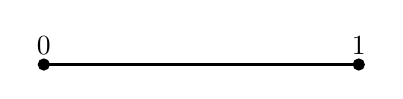
\begin{tikzpicture}[] % Line
         \draw[thick](0,0) -- (4,0);
             \filldraw(0,0) circle (2pt);
             \filldraw(4,0) circle (2pt);
         \node[above] at (0,0){0};
         \node[above] at (4,0){1};
      \end{tikzpicture}
     \hspace{1cm}
     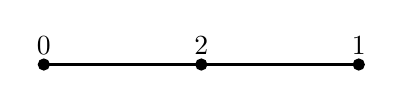
\begin{tikzpicture}[] % Line
         \draw[thick](0,0) -- (4,0);
             \filldraw(0,0) circle (2pt);
             \filldraw(4,0) circle (2pt);
             \filldraw(2,0) circle (2pt);
         \node[above] at (0,0){0};
         \node[above] at (4,0){1};
         \node[above] at (2,0){2};
      \end{tikzpicture}
     \end{center}
  \begin{center}  (a) \hspace{5cm} (b) \end{center}
  \caption{(a) Base line {\tt (line<2>)} and (b) extended line {\tt (line<3>)} topology in Shards.}
  \label{fig:line}
 \end{figure}

\subsection{Triangle}

A triangle is an object of dimension two with three vertices and three edges. The base and extended topologies available in Shards are shown in Figure \ref{fig:tri1}. The edge numbering is shown in Figure \ref{fig:tri2}.

% Triangle Node Numbering
\begin{figure}[ht]
  \begin{center}
   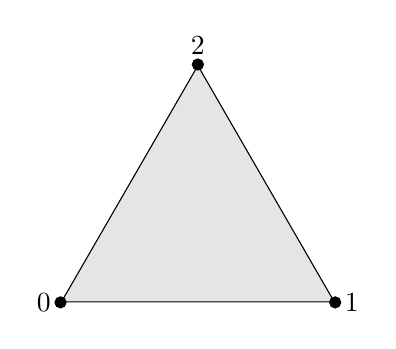
\begin{tikzpicture} % 3 nodes
      \node[name=p3, regular polygon,regular polygon sides=3, minimum size=4cm, draw, fill=black!10]{};
      \filldraw(p3.corner 1) circle (2pt);
      \filldraw(p3.corner 2) circle (2pt);
      \filldraw(p3.corner 3) circle (2pt);
      \node[above] at (p3.corner 1){2};
      \node[left] at (p3.corner 2){0};
      \node[right] at (p3.corner 3){1};
   \end{tikzpicture}
   \hspace{1cm}
   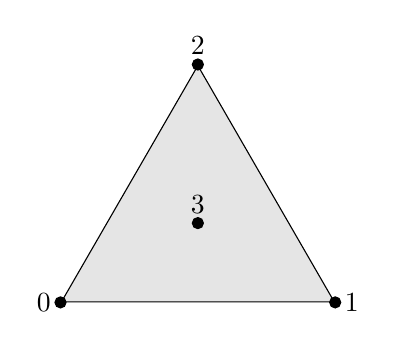
\begin{tikzpicture} % 4 nodes
      \node[name=p3, regular polygon,regular polygon sides=3, minimum size=4cm, draw,  fill=black!10]{};
      \filldraw(p3.corner 1) circle (2pt);
      \filldraw(p3.corner 2) circle (2pt);
      \filldraw(p3.corner 3) circle (2pt);
      \filldraw(p3.center) circle (2pt);
      \node[above] at (p3.corner 1){2};
      \node[left] at (p3.corner 2){0};
      \node[right] at (p3.corner 3){1};
      \node[above] at (p3.center){3};
   \end{tikzpicture}
  \end{center}
  \begin{center}  (a) \hspace{5cm} (b) \end{center}
  \begin{center}
   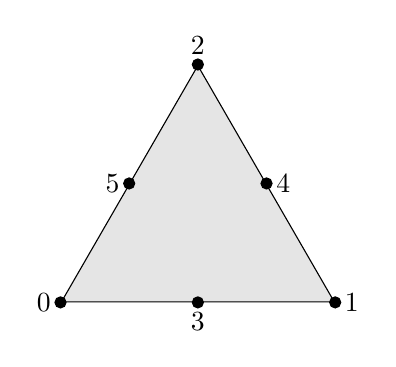
\begin{tikzpicture} % 6 nodes
      \node[name=p3, regular polygon,regular polygon sides=3, minimum size=4cm, draw,  fill=black!10]{};
      \filldraw(p3.corner 1) circle (2pt);
      \filldraw(p3.corner 2) circle (2pt);
      \filldraw(p3.corner 3) circle (2pt);
      \filldraw(p3.side 1) circle (2pt);
      \filldraw(p3.side 2) circle (2pt);
      \filldraw(p3.side 3) circle (2pt);
      \node[above] at (p3.corner 1){2};
      \node[left] at (p3.corner 2){0};
      \node[right] at (p3.corner 3){1};
      \node[left] at (p3.side 1){5};
      \node[below] at (p3.side 2){3};
      \node[right] at (p3.side 3){4};
   \end{tikzpicture}
  \end{center}
  \begin{center} (c) \end{center}
  \caption{(a) Base triangle {\tt (Triangle<>)}, (b) four-node extended triangle {\tt (Triangle<4>)},  and (c) six-node extended triangle {\tt (Triangle<6>)} topology in Shards.} 
 \label{fig:tri1}
\end{figure}

% Triangle Edge Numbering
\begin{figure}[ht]
  \begin{center}
    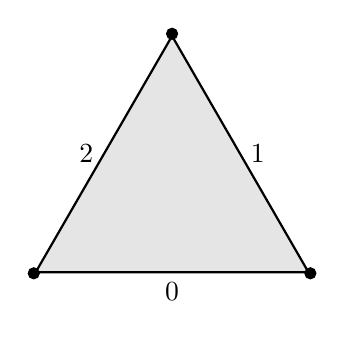
\begin{tikzpicture}
      \node[name=p3, regular polygon,regular polygon sides=3, minimum size=4cm, draw, thick, fill=black!10]{};
      \node[left] at (p3.side 1){2};
      \node[below] at (p3.side 2){0};
      \node[right] at (p3.side 3){1};
      \filldraw(p3.corner 1) circle (2pt);
      \filldraw(p3.corner 2) circle (2pt);
      \filldraw(p3.corner 3) circle (2pt);
    \end{tikzpicture}
  \end{center}
 \caption{Triangle edge (1-cell) numbering in Shards.}
\label{fig:tri2}
\end{figure}


\subsection{Quadrilateral}
A quadrilateral is an object of dimension two with four vertices and four edges. The base and extended topologies available in Shards are shown in Figure \ref{fig:quad1}. The edge numbering is shown in Figure \ref{fig:quad2}.
% Quadrilateral Node Numbering
\begin{figure}[ht]
 \begin{center}
   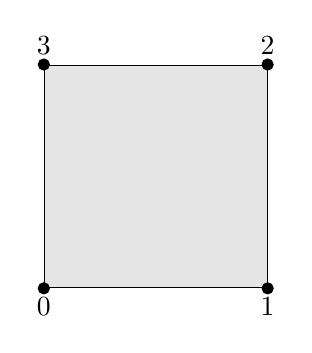
\begin{tikzpicture}
      \node[name=p4, regular polygon,regular polygon sides=4, minimum size=4cm, draw, fill=black!10]{};
      \filldraw(p4.corner 1) circle (2pt);
      \filldraw(p4.corner 2) circle (2pt);
      \filldraw(p4.corner 3) circle (2pt);
      \filldraw(p4.corner 4) circle (2pt);
      \node[above] at (p4.corner 1){2};
      \node[above] at (p4.corner 2){3};
      \node[below] at (p4.corner 3){0};
      \node[below] at (p4.corner 4){1};
   \end{tikzpicture}
   \hspace{1cm}
   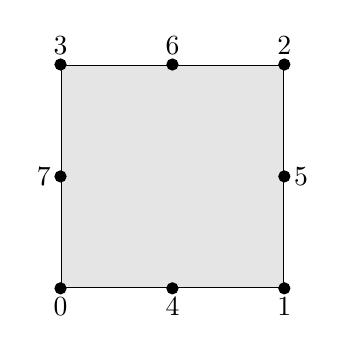
\begin{tikzpicture}
      \node[name=p4, regular polygon,regular polygon sides=4, minimum size=4cm, draw, fill=black!10]{};
      \filldraw(p4.corner 1) circle (2pt);
      \filldraw(p4.corner 2) circle (2pt);
      \filldraw(p4.corner 3) circle (2pt);
      \filldraw(p4.corner 4) circle (2pt);
      \filldraw(p4.side 1) circle (2pt);
      \filldraw(p4.side 2) circle (2pt);
      \filldraw(p4.side 3) circle (2pt);
      \filldraw(p4.side 4) circle (2pt);
      \node[above] at (p4.corner 1){2};
      \node[above] at (p4.corner 2){3};
      \node[below] at (p4.corner 3){0};
      \node[below] at (p4.corner 4){1};
      \node[above] at (p4.side 1){6};
      \node[left] at (p4.side 2){7};
      \node[below] at (p4.side 3){4};
      \node[right] at (p4.side 4){5};
   \end{tikzpicture}
   \hspace{1cm}
   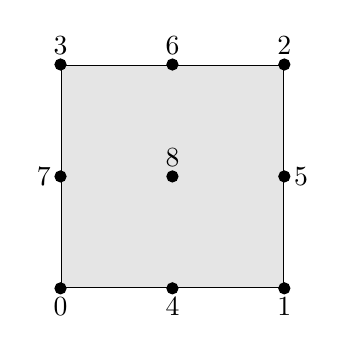
\begin{tikzpicture}
      \node[name=p4, regular polygon,regular polygon sides=4, minimum size=4cm, draw, fill=black!10]{};
      \filldraw(p4.corner 1) circle (2pt);
      \filldraw(p4.corner 2) circle (2pt);
      \filldraw(p4.corner 3) circle (2pt);
      \filldraw(p4.corner 4) circle (2pt);
      \filldraw(p4.side 1) circle (2pt);
      \filldraw(p4.side 2) circle (2pt);
      \filldraw(p4.side 3) circle (2pt);
      \filldraw(p4.side 4) circle (2pt);
      \filldraw(p4.center) circle (2pt);
      \node[above] at (p4.corner 1){2};
      \node[above] at (p4.corner 2){3};
      \node[below] at (p4.corner 3){0};
      \node[below] at (p4.corner 4){1};
      \node[above] at (p4.side 1){6};
      \node[left] at (p4.side 2){7};
      \node[below] at (p4.side 3){4};
      \node[right] at (p4.side 4){5};
      \node[above] at (p4.center){8};
   \end{tikzpicture}
 \end{center}
  \begin{center} (a) \hspace{4cm} (b) \hspace{4cm} (c) \end{center}
 \caption{(a) Base quadrilateral {\tt (Quadrilateral<4>)}, (b) eight-node extended quadrilateral {\tt (Quadrilateral<8>)}, and (c) nine-node extended quadrilateral {\tt (Quadrilateral<9>)} topology in Shards.}
\label{fig:quad1}
\end{figure}

% Quadrilateral Edge
\begin{figure}[ht]
 \begin{center}
  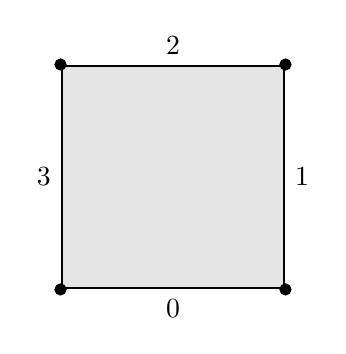
\begin{tikzpicture}
     \node[name=p4, regular polygon,regular polygon sides=4, minimum size=4cm, draw, thick, fill=black!10]{};
      \filldraw(p4.corner 1) circle (2pt);
      \filldraw(p4.corner 2) circle (2pt);
      \filldraw(p4.corner 3) circle (2pt);
      \filldraw(p4.corner 4) circle (2pt);
     \node[above] at (p4.side 1){2};
     \node[left] at (p4.side 2){3};
     \node[below] at (p4.side 3){0};
     \node[right] at (p4.side 4){1};
  \end{tikzpicture}
 \end{center}
 \caption{Quadrilateral edge (1-cell) numbering in Shards.}
\label{fig:quad2}
\end{figure}

\subsection{Pentagon}
 
A pentagon is an object of dimension two with five vertices and five edges. Only a base topology is provided for a pentagon in Shards, which is shown in Figure \ref{fig:pent} along with the edge numbering.
\begin{figure}[ht]
 \begin{center}
   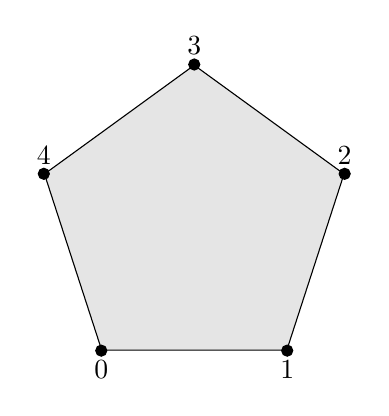
\begin{tikzpicture}
      \node[name=p5, regular polygon,regular polygon sides=5, minimum size=4cm, draw, fill=black!10]{};
      \filldraw(p5.corner 1) circle (2pt);
      \filldraw(p5.corner 2) circle (2pt);
      \filldraw(p5.corner 3) circle (2pt);
      \filldraw(p5.corner 4) circle (2pt);
      \filldraw(p5.corner 5) circle (2pt);
      \node[below] at (p5.corner 3){0};
      \node[below] at (p5.corner 4){1};
      \node[above] at (p5.corner 5){2};
      \node[above] at (p5.corner 1){3};
      \node[above] at (p5.corner 2){4};
   \end{tikzpicture}
   \hspace{2cm}
   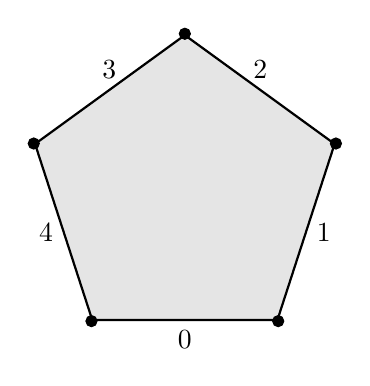
\begin{tikzpicture}
      \node[name=p5, regular polygon,regular polygon sides=5, minimum size=4cm, draw, thick, fill=black!10]{};
      \filldraw(p5.corner 1) circle (2pt);
      \filldraw(p5.corner 2) circle (2pt);
      \filldraw(p5.corner 3) circle (2pt);
      \filldraw(p5.corner 4) circle (2pt);
      \filldraw(p5.corner 5) circle (2pt);
      \node[below] at (p5.side 3){0};
      \node[right] at (p5.side 4){1};
      \node[above] at (p5.side 5){2};
      \node[above] at (p5.side 1){3};
      \node[left] at (p5.side 2){4};
   \end{tikzpicture}  
  \end{center}
  \begin{center} (a) \hspace{5cm} (b) \end{center}
  \caption{ (a) Base pentagon ({\tt Pentagon<>}) topology and (b) edge (1-cell) numbering in Shards.}
 \label{fig:pent}
 \end{figure}
   
\subsection{Hexagon}
A hexagon is an object of dimension two with six vertices and six edges. Only a base topology is provided for a hexagon in Shards, which is shown in Figure \ref{fig:hex} along with the edge numbering.
\begin{figure}[ht]
  \begin{center}
   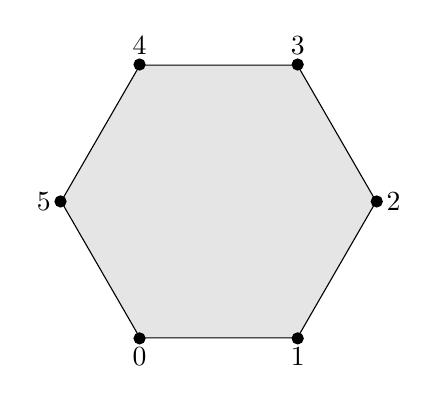
\begin{tikzpicture}
      \node[name=p6, regular polygon,regular polygon sides=6, minimum size=4cm, draw, fill=black!10]{};
      \filldraw(p6.corner 1) circle (2pt);
      \filldraw(p6.corner 2) circle (2pt);
      \filldraw(p6.corner 3) circle (2pt);
      \filldraw(p6.corner 4) circle (2pt);
      \filldraw(p6.corner 5) circle (2pt);
      \filldraw(p6.corner 6) circle (2pt);
      \node[left] at (p6.corner 3){5};
      \node[below] at (p6.corner 4){0};
      \node[below] at (p6.corner 5){1};
      \node[above] at (p6.corner 1){3};
      \node[above] at (p6.corner 2){4};
      \node[right] at (p6.corner 6){2};
    \end{tikzpicture}
    \hspace{2cm}
    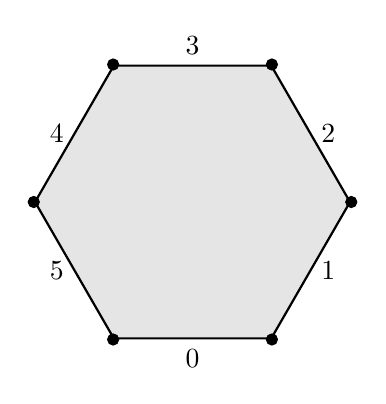
\begin{tikzpicture}
      \node[name=p6, regular polygon,regular polygon sides=6, minimum size=4cm, draw, thick, fill=black!10]{};
      \filldraw(p6.corner 1) circle (2pt);
      \filldraw(p6.corner 2) circle (2pt);
      \filldraw(p6.corner 3) circle (2pt);
      \filldraw(p6.corner 4) circle (2pt);
      \filldraw(p6.corner 5) circle (2pt);
      \filldraw(p6.corner 6) circle (2pt);
      \node[left] at (p6.side 3){5};
      \node[below] at (p6.side 4){0};
      \node[right] at (p6.side 5){1};
      \node[above] at (p6.side 1){3};
      \node[left] at (p6.side 2){4};
      \node[right] at (p6.side 6){2};
    \end{tikzpicture}
  \end{center}
 \begin{center} 
     \hspace{1cm} (a) \hspace{5cm} (b)  \\
   \caption{ (a) Base hexagon ({\tt Hexagon<>}) topology and (b) edge (1-cell) numbering in Shards.}
 \end{center}
\label{fig:hex}
\end{figure}

% Tetrahedron Node Numbering
\subsection{Tetrahedron}
A tetrahedron is an object of dimension three with four vertices, six edges, and four sides. The base and extended topologies available in Shards are shown in Figure \ref{fig:tet1}. The edge numbering is shown in Figure \ref{fig:tet2} and the face numbering in Figure \ref{fig:tet3}.
 \begin{figure}[ht]
  \begin{center}
    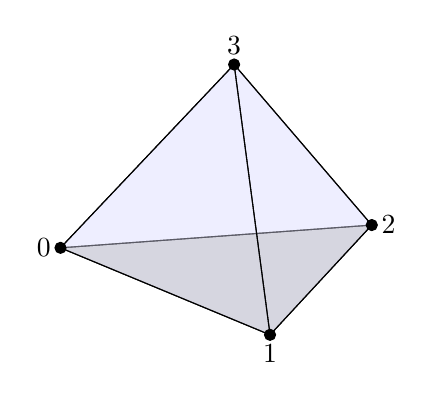
\begin{tikzpicture}[join=round] % tet with 4 nodes
        \filldraw[fill=black!20](1.748,.561)--(-2.205,.272)--(.456,-.833)--cycle;
        \filldraw[fill=blue!10,fill opacity=0.4](0,2.6)--(-2.205,.272)--(1.748,.561)--(0,2.6)--cycle;
        \filldraw[fill=blue!10,fill opacity=0.4](0,2.6)--(1.748,.561)--(.456,-.833)--(0,2.6)--cycle;
        \filldraw[fill=blue!10,fill opacity=0.4](0,2.6)--(.456,-.833)--(-2.205,.272)--(0,2.6)--cycle;
        \filldraw(1.748,.561) circle (2pt);
        \filldraw(-2.205,.272) circle (2pt);
        \filldraw(0,2.6) circle (2pt);
        \filldraw(.456,-.833) circle (2pt);
        \fill[black]
                (-2.205,.272) node [left] {0}
                (.456,-.833) node [below] {1}
                (1.748,.561) node [right] {2}
                (0,2.6) node [above] {3};
    \end{tikzpicture}
     \hspace{1cm}
    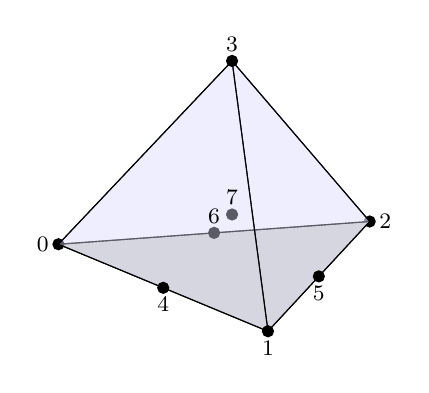
\begin{tikzpicture}[join=round] % tet with 8 nodes
        \filldraw(1.748,.561) circle (2pt);
        \filldraw[fill=black!20](1.748,.561)--(-2.205,.272)--(.456,-.833)--cycle;
        \filldraw[fill=blue!10,fill opacity=0.4](0,2.6)--(-2.205,.272)--(1.748,.561)--(0,2.6)--cycle;
        \filldraw[fill=blue!10,fill opacity=0.4](0,2.6)--(1.748,.561)--(.456,-.833)--(0,2.6)--cycle;
        \filldraw(-.228,.417) circle (2pt);
        \filldraw(-2.205,.272) circle (2pt);
        \filldraw(0,.65) circle (2pt);
        \filldraw[fill=blue!10,fill opacity=0.4](0,2.6)--(.456,-.833)--(-2.205,.272)--(0,2.6)--cycle;
        \filldraw(1.102,-.136) circle (2pt);
        \filldraw(-.874,-.281) circle (2pt);
        \filldraw(0,2.6) circle (2pt);
        \filldraw(.456,-.833) circle (2pt);
        \fill[black,font=\footnotesize]
                (-2.205,.272) node [left] {0}
                (.456,-.833) node [below] {1}
                (1.748,.561) node [right] {2}
                (0,2.6) node [above] {3}
                (-.874,-.281) node [below] {4}
                (1.102,-.136) node [below] {5}
                (-.228,.417) node [above] {6}
                (0,.65) node [above] {7};
     \end{tikzpicture}
   \end{center}
   \begin{center} {(a) \hspace{5cm} (b)}  \end{center}
   \begin{center}
    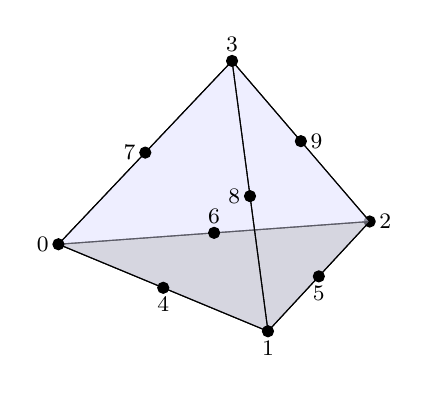
\begin{tikzpicture}[join=round]% tet with 10 nodes
        \filldraw[fill=black!20](1.748,.561)--(-2.205,.272)--(.456,-.833)--cycle;
        \filldraw(1.748,.561) circle (2pt);
        \filldraw[fill=blue!10,fill opacity=0.4](0,2.6)--(-2.205,.272)--(1.748,.561)--(0,2.6)--cycle;
        \filldraw[fill=blue!10,fill opacity=0.4](0,2.6)--(1.748,.561)--(.456,-.833)--(0,2.6)--cycle;
        \filldraw[fill=blue!10,fill opacity=0.4](0,2.6)--(.456,-.833)--(-2.205,.272)--(0,2.6)--cycle;
        \filldraw(-.228,.417) circle (2pt);
        \filldraw(-2.205,.272) circle (2pt);
        \filldraw(.874,1.581) circle (2pt);
        \filldraw(-1.102,1.436) circle (2pt);
        \filldraw(1.102,-.136) circle (2pt);
        \filldraw(-.874,-.281) circle (2pt);
        \filldraw(0,2.6) circle (2pt);
        \filldraw(.228,.883) circle (2pt);
        \filldraw(.456,-.833) circle (2pt);
        \fill[black,font=\footnotesize]
                (-2.205,.272) node [left] {0}
                (.456,-.833) node [below] {1}
                (1.748,.561) node [right] {2}
                (0,2.6) node [above] {3}
                (-.874,-.281) node [below] {4}
                (1.102,-.136) node [below] {5}
                (-.228,.417) node [above] {6}
                (-1.102,1.436) node [left] {7}
                (.228,.883) node [left] {8}
                (.874,1.581) node [right] {9};
     \end{tikzpicture}
    \end{center}
  \begin{center}(c)\end{center}
   \caption{(a) Base tetrahedron {\tt (Tetrahedron<>)}, (b) eight-node extended tetrahedron {\tt (Tetrahedron<8>)}, and (e) ten-node extended tetrahedron {\tt (Tetrahedron<10>)} topology in Shards.}
 \label{fig:tet1}
\end{figure}

\begin{figure}[ht]
 \begin{center}
   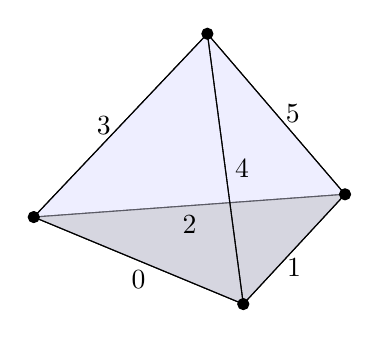
\begin{tikzpicture}[join=round] % Tetrahedron edges
        \filldraw[fill=blue!10,fill opacity=0.4](0,2.6)--(-2.205,.272)--(1.748,.561)--(0,2.6)--cycle;
        \filldraw[fill=black!20](1.748,.561)--(-2.205,.272)--(.456,-.833)--cycle;
        \filldraw[fill=blue!10,fill opacity=0.4](0,2.6)--(1.748,.561)--(.456,-.833)--(0,2.6)--cycle;
        \filldraw[fill=blue!10,fill opacity=0.4](0,2.6)--(.456,-.833)--(-2.205,.272)--(0,2.6)--cycle;
        \filldraw(1.748,.561) circle (2pt);
        \filldraw(-2.205,.272) circle (2pt);
        \filldraw(0,2.6) circle (2pt);
        \filldraw(.456,-.833) circle (2pt);
        \fill[black]
                (-.874,-.281) node [below] {0}
                (1.102,-.136) node [below] {1}
                (-.228,.417) node [below] {2}
                (-1.102,1.436) node [left] {3}
                (.228,.883) node [right] {4}
                (.874,1.581) node [right] {5};
   \end{tikzpicture}
  \end{center}
 \caption{Tetrahedron edge (1-cell) numbering in Shards.}
 \label{fig:tet2}
\end{figure}

\begin{figure}[ht]
 \begin{center}
  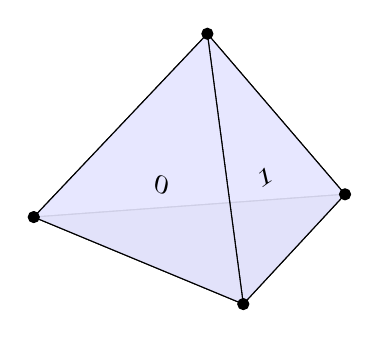
\begin{tikzpicture}[join=round] % Tetrahedron faces
       \filldraw[fill=blue!10,fill opacity=0.4](0,2.6)--(-2.205,.272)--(1.748,.561)--(0,2.6)--cycle;
       \filldraw[fill=black!20](1.748,.561)--(-2.205,.272)--(.456,-.833)--cycle;
       \filldraw[fill=blue!10,fill opacity=0.9](0,2.6)--(1.748,.561)--(.456,-.833)--(0,2.6)--cycle;
       \filldraw[fill=blue!10,fill opacity=0.9](0,2.6)--(.456,-.833)--(-2.205,.272)--(0,2.6)--cycle;
        \filldraw(1.748,.561) circle (2pt);
        \filldraw(-2.205,.272) circle (2pt);
        \filldraw(0,2.6) circle (2pt);
        \filldraw(.456,-.833) circle (2pt);
       \fill[black]
                (-.583,.68) node [yslant=-.5,xslant=.2] {0}
                (.735,.776) node [yslant=.7,xslant=-.2] {1};
   \end{tikzpicture}
  \hspace{1cm}
  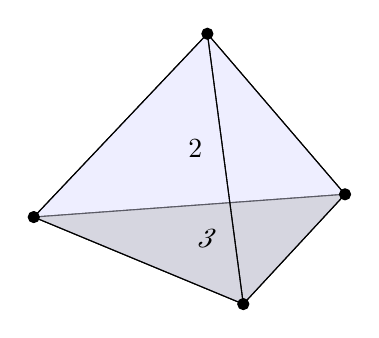
\begin{tikzpicture}[join=round] % Tetrahedron faces
       \filldraw[fill=blue!10,fill opacity=0.4](0,2.6)--(-2.205,.272)--(1.748,.561)--(0,2.6)--cycle;
       \filldraw[fill=black!20](1.748,.561)--(-2.205,.272)--(.456,-.833)--cycle;
       \filldraw[fill=blue!10,fill opacity=0.4](0,2.6)--(1.748,.561)--(.456,-.833)--(0,2.6)--cycle;
       \filldraw[fill=blue!10,fill opacity=0.4](0,2.6)--(.456,-.833)--(-2.205,.272)--(0,2.6)--cycle;
        \filldraw(1.748,.561) circle (2pt);
        \filldraw(-2.205,.272) circle (2pt);
        \filldraw(0,2.6) circle (2pt);
        \filldraw(.456,-.833) circle (2pt);
       \fill[black]
                (-.152,1.144) node [] {2}
                (0,0) node [xslant=.5,yslant=0.0] {3};
   \end{tikzpicture}
 \end{center}
 \caption{Tetrahedron face (2-cell) numbering in Shards.}
 \label{fig:tet3}
\end{figure}


\subsection{Pyramid}
A pyramid is an object of dimension three with five vertices, eight edges, and five sides. The base and extended topologies available in Shards are shown in Figure \ref{fig:pyr1}. The edge numbering is shown in Figure \ref{fig:pyr2} and the face numbering in Figure \ref{fig:pyr3}.

\begin{figure}[ht]
 \begin{center}
    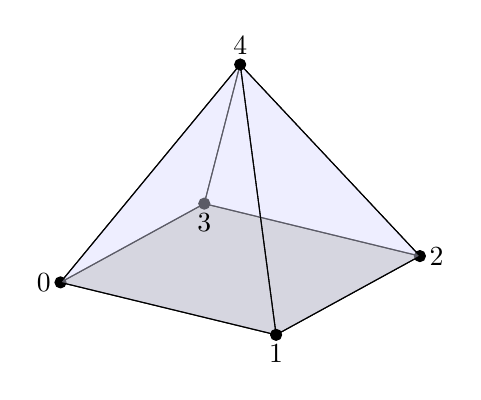
\begin{tikzpicture}[join=round] % pyramid with 5 nodes
       \filldraw[fill=black!20](2.282,.167)--(-.456,.833)--(-2.282,-.167)--(.456,-.833)--cycle;
       \filldraw[fill=blue!10,fill opacity=0.4](0,2.6)--(-2.282,-.167)--(-.456,.833)--(0,2.6)--cycle;
       \filldraw[fill=blue!10,fill opacity=0.4](0,2.6)--(-.456,.833)--(2.282,.167)--(0,2.6)--cycle;
       \filldraw(-.456,.833) circle (2pt);
       \filldraw(2.282,.167) circle (2pt);
       \filldraw[fill=blue!10,fill opacity=0.4](0,2.6)--(2.282,.167)--(.456,-.833)--(0,2.6)--cycle;
       \filldraw(-2.282,-.167) circle (2pt);
       \filldraw[fill=blue!10,fill opacity=0.4](0,2.6)--(.456,-.833)--(-2.282,-.167)--(0,2.6)--cycle;
       \filldraw(0,2.6) circle (2pt);
       \filldraw(.456,-.833) circle (2pt);
       \fill[black]
                (-2.282,-.167) node [left] {0}
                (.456,-.833) node [below] {1}
                (2.282,.167) node [right] {2}
                (-.456,.833) node [below] {3}
                (0,2.6) node [above] {4};
   \end{tikzpicture}
   \hspace{1cm}
   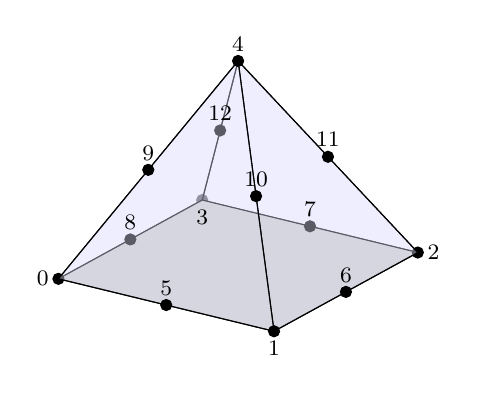
\begin{tikzpicture}[join=round] % pyramid with 13 nodes
        \filldraw(-.456,.833) circle (2pt);
        \filldraw[fill=blue!10,fill opacity=0.4](0,2.6)--(-.456,.833)--(2.282,.167)--(0,2.6)--cycle;
        \filldraw[fill=blue!10,fill opacity=0.4](0,2.6)--(-2.282,-.167)--(-.456,.833)--(0,2.6)--cycle;
        \filldraw[fill=black!20](2.282,.167)--(-.456,.833)--(-2.282,-.167)--(.456,-.833)--cycle;
        \filldraw(.913,.5) circle (2pt);
        \filldraw(-1.369,.333) circle (2pt);
        \filldraw(-.228,1.717) circle (2pt);
        \filldraw(2.282,.167) circle (2pt);
        \filldraw[fill=blue!10,fill opacity=0.4](0,2.6)--(2.282,.167)--(.456,-.833)--(0,2.6)--cycle;
        \filldraw(1.141,1.383) circle (2pt);
        \filldraw(-2.282,-.167) circle (2pt);
        \filldraw[fill=blue!10,fill opacity=0.4](0,2.6)--(.456,-.833)--(-2.282,-.167)--(0,2.6)--cycle;
        \filldraw(-1.141,1.217) circle (2pt);
        \filldraw(1.369,-.333) circle (2pt);
        \filldraw(0,2.6) circle (2pt);
        \filldraw(-.913,-.5) circle (2pt);
        \filldraw(.228,.883) circle (2pt);
        \filldraw(.456,-.833) circle (2pt);
        \fill[black,font=\footnotesize]
                (-2.282,-.167) node [left] {0}
                (.456,-.833) node [below] {1}
                (2.282,.167) node [right] {2}
                (-.456,.833) node [below] {3}
                (0,2.6) node [above] {4}
                (-.913,-.5) node [above] {5}
                (1.369,-.333) node [above] {6}
                (.913,.5) node [above] {7}
                (-1.369,.333) node [above] {8}
                (-1.141,1.217) node [above] {9}
                (.228,.883) node [above] {10}
                (1.141,1.383) node [above] {11}
                (-.228,1.717) node [above] {12};
   \end{tikzpicture}
 \end{center}
 \begin{center}{(a) \hspace{5cm} (b)} \end{center}
 \begin{center}
    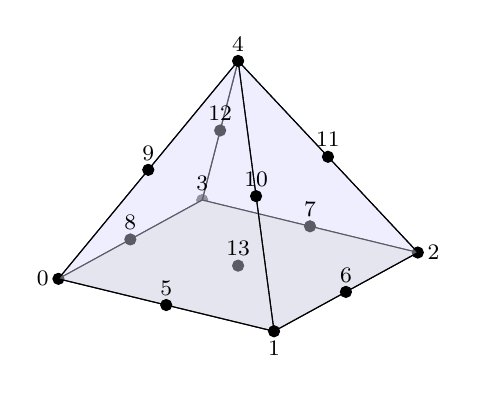
\begin{tikzpicture}[join=round] %pyramid with 14 nodes
         \filldraw(-.456,.833) circle (2pt);
         \filldraw[fill=blue!10,fill opacity=0.4](0,2.6)--(-.456,.833)--(2.282,.167)--(0,2.6)--cycle;
         \filldraw[fill=blue!10,fill opacity=0.4](0,2.6)--(-2.282,-.167)--(-.456,.833)--(0,2.6)--cycle;
         \filldraw[fill=black!10](2.282,.167)--(-.456,.833)--(-2.282,-.167)--(.456,-.833)--cycle;
         \filldraw(.913,.5) circle (2pt);
         \filldraw(-1.369,.333) circle (2pt);
         \filldraw(-.228,1.717) circle (2pt);
         \filldraw(2.282,.167) circle (2pt);
         \filldraw[fill=blue!10,fill opacity=0.4](0,2.6)--(2.282,.167)--(.456,-.833)--(0,2.6)--cycle;
         \filldraw(0,0) circle (2pt);
         \filldraw(1.141,1.383) circle (2pt);
         \filldraw(-2.282,-.167) circle (2pt);
         \filldraw[fill=blue!10,fill opacity=0.4](0,2.6)--(.456,-.833)--(-2.282,-.167)--(0,2.6)--cycle;
         \filldraw(-1.141,1.217) circle (2pt);
         \filldraw(1.369,-.333) circle (2pt);
         \filldraw(0,2.6) circle (2pt);
         \filldraw(-.913,-.5) circle (2pt);
         \filldraw(.228,.883) circle (2pt);
         \filldraw(.456,-.833) circle (2pt);
         \fill[black,font=\footnotesize]
                (-2.282,-.167) node [left] {0}
                (.456,-.833) node [below] {1}
                (2.282,.167) node [right] {2}
                (-.456,.833) node [above] {3}
                (0,2.6) node [above] {4}
                (-.913,-.5) node [above] {5}
                (1.369,-.333) node [above] {6}
                (.913,.5) node [above] {7}
                (-1.369,.333) node [above] {8}
                (-1.141,1.217) node [above] {9}
                (.228,.883) node [above] {10}
                (1.141,1.383) node [above] {11}
                (-.228,1.717) node [above] {12}
                (0,0) node [above] {13};
    \end{tikzpicture}
 \end{center}
 \begin{center}(c)\end{center}
  \caption{(a) Base pyramid {\tt (Pyramid<>)}, (b) thirteen-node extended pyramid {\tt (Pyramid<13>)}, and (c) fourteen-node extended pyramid {\tt (Pyramid<14>)} topology in Shards.}
 \label{fig:pyr1}
\end{figure}

\begin{figure}[ht]
 \begin{center}
   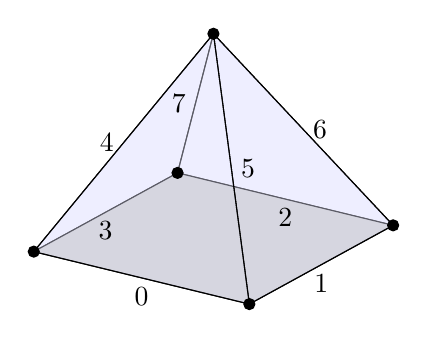
\begin{tikzpicture}[join=round] % Pyramid edges
       \filldraw[fill=blue!10,fill opacity=0.4](0,2.6)--(-2.282,-.167)--(-.456,.833)--(0,2.6)--cycle;
       \filldraw[fill=blue!10,fill opacity=0.4](0,2.6)--(-.456,.833)--(2.282,.167)--(0,2.6)--cycle;
       \filldraw[fill=black!20](2.282,.167)--(-.456,.833)--(-2.282,-.167)--(.456,-.833)--cycle;
       \filldraw[fill=blue!10,fill opacity=0.4](0,2.6)--(2.282,.167)--(.456,-.833)--(0,2.6)--cycle;
       \filldraw[fill=blue!10,fill opacity=0.4](0,2.6)--(.456,-.833)--(-2.282,-.167)--(0,2.6)--cycle;
       \filldraw(-.456,.833) circle (2pt);
       \filldraw(2.282,.167) circle (2pt);
       \filldraw(-2.282,-.167) circle (2pt);
       \filldraw(0,2.6) circle (2pt);
       \filldraw(.456,-.833) circle (2pt);
       \fill[black]
                (-.913,-.5) node [below] {0}
                (1.369,-.333) node [below] {1}
                (.913,.5) node [below] {2}
                (-1.369,.333) node [below] {3}
                (-1.141,1.217) node [left] {4}
                (.228,.883) node [right] {5}
                (1.141,1.383) node [right] {6}
                (-.228,1.717) node [left] {7};
   \end{tikzpicture}
  \end{center}
  \caption{Pyramid edge (1-cell) numbering in Shards.}
 \label{fig:pyr2}
\end{figure}
  
\begin{figure}[ht]
 \begin{center}
   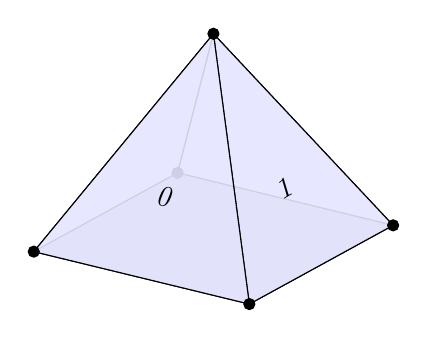
\begin{tikzpicture}[join=round] % Pyramid Faces
       \filldraw[fill=blue!10,fill opacity=0.4](0,2.6)--(-2.282,-.167)--(-.456,.833)--(0,2.6)--cycle;
       \filldraw[fill=blue!10,fill opacity=0.4](0,2.6)--(-.456,.833)--(2.282,.167)--(0,2.6)--cycle;
       \filldraw[fill=black!20](2.282,.167)--(-.456,.833)--(-2.282,-.167)--(.456,-.833)--cycle;
       \filldraw(-.456,.833) circle (2pt);
       \filldraw[fill=blue!10,fill opacity=0.9](0,2.6)--(2.282,.167)--(.456,-.833)--(0,2.6)--cycle;
       \filldraw[fill=blue!10,fill opacity=0.9](0,2.6)--(.456,-.833)--(-2.282,-.167)--(0,2.6)--cycle;
       \filldraw(2.282,.167) circle (2pt);
       \filldraw(-2.282,-.167) circle (2pt);
       \filldraw(0,2.6) circle (2pt);
       \filldraw(.456,-.833) circle (2pt);
       \fill[black]
                (-.609,.533) node [xslant=.4,yslant=-0.2] {0}
                (.913,.644) node [xslant=-.3,yslant=.5] {1};
   \end{tikzpicture}
  \hspace{1cm}
   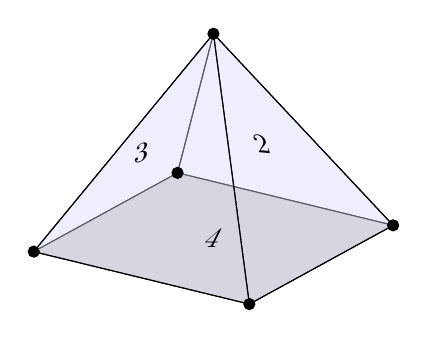
\begin{tikzpicture}[join=round] % Pyramid Faces
       \filldraw[fill=blue!10,fill opacity=0.4](0,2.6)--(-2.282,-.167)--(-.456,.833)--(0,2.6)--cycle;
       \filldraw[fill=blue!10,fill opacity=0.4](0,2.6)--(-.456,.833)--(2.282,.167)--(0,2.6)--cycle;
       \filldraw[fill=black!20](2.282,.167)--(-.456,.833)--(-2.282,-.167)--(.456,-.833)--cycle;
       \filldraw[fill=blue!10,fill opacity=0.4](0,2.6)--(2.282,.167)--(.456,-.833)--(0,2.6)--cycle;
       \filldraw[fill=blue!10,fill opacity=0.4](0,2.6)--(.456,-.833)--(-2.282,-.167)--(0,2.6)--cycle;
       \filldraw(-.456,.833) circle (2pt);
       \filldraw(2.282,.167) circle (2pt);
       \filldraw(-2.282,-.167) circle (2pt);
       \filldraw(0,2.6) circle (2pt);
       \filldraw(.456,-.833) circle (2pt);
       \fill[black]
                (.609,1.2) node [xslant=-0.4,yslant=-.1] {2}
                (-.913,1.089) node [xslant=.1,yslant=.4] {3}
                (0,0) node [xslant=.5] {4};
   \end{tikzpicture}
 \end{center}
 \caption{Pyramid face (2-cell) numbering in Shards.}
 \label{fig:pyr3}
\end{figure}


% Wedge Node Numbering
\subsection{Wedge}
A wedge is an object of dimension three with six vertices, nine edges, and five sides. The base and extended topologies available in Shards are shown in Figure \ref{fig:wed1}. The edge numbering is shown in Figure \ref{fig:wed2} and the face numbering in Figure \ref{fig:wed3}.
 \begin{figure}[ht]
  \begin{center}
    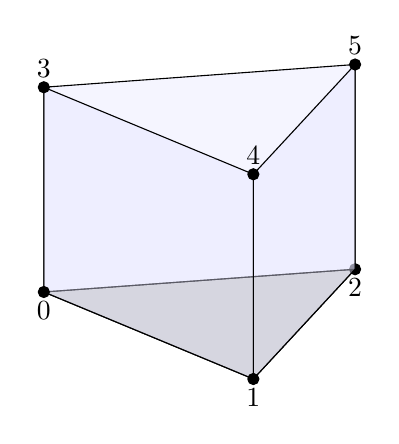
\begin{tikzpicture}[join=round] %Wedge with 6 nodes
        \filldraw[fill=black!20](1.748,.561)--(-2.205,.272)--(.456,-.833)--cycle;
        \filldraw(1.748,.561) circle (2pt);
        \filldraw[fill=blue!10,fill opacity=0.4](-2.205,2.872)--(-2.205,.272)--(1.748,.561)--(1.748,3.161)--cycle;
        \filldraw[fill=blue!10,fill opacity=0.4](1.748,3.161)--(1.748,.561)--(.456,-.833)--(.456,1.767)--cycle;
        \filldraw[fill=blue!10,fill opacity=0.4](.456,1.767)--(.456,-.833)--(-2.205,.272)--(-2.205,2.872)--cycle;
        \filldraw(-2.205,.272) circle (2pt);
        \filldraw(1.748,3.161) circle (2pt);
        \filldraw(-2.205,2.872) circle (2pt);
        \filldraw(.456,-.833) circle (2pt);
        \filldraw(.456,1.767) circle (2pt);
        \fill[black]
                (-2.205,.272) node [below] {0}
                (.456,-.833) node [below] {1}
                (1.748,.561) node [below] {2}
                (-2.205,2.872) node [above] {3}
                (.456,1.767) node [above] {4}
                (1.748,3.161) node [above] {5};
    \end{tikzpicture}
     \hspace{1cm}
     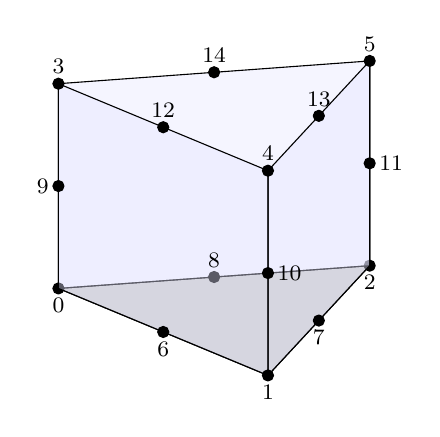
\begin{tikzpicture}[join=round]
         \filldraw[fill=black!20](1.748,.561)--(-2.205,.272)--(.456,-.833)--cycle;
         \filldraw(1.748,.561) circle (2pt);
         \filldraw[fill=blue!10,fill opacity=0.4](-2.205,2.872)--(-2.205,.272)--(1.748,.561)--(1.748,3.161)--cycle;
         \filldraw[fill=blue!10,fill opacity=0.4](1.748,3.161)--(1.748,.561)--(.456,-.833)--(.456,1.767)--cycle;
         \filldraw(-.228,.417) circle (2pt);
         \filldraw(1.748,1.861) circle (2pt);
         \filldraw(-2.205,.272) circle (2pt);
         \filldraw[fill=blue!10,fill opacity=0.4](.456,1.767)--(.456,-.833)--(-2.205,.272)--(-2.205,2.872)--cycle;
         \filldraw(1.748,3.161) circle (2pt);
         \filldraw(-2.205,1.572) circle (2pt);
         \filldraw(-.228,3.017) circle (2pt);
         \filldraw(-2.205,2.872) circle (2pt);
         \filldraw(1.102,-.136) circle (2pt);
         \filldraw(-.874,-.281) circle (2pt);
         \filldraw(1.102,2.464) circle (2pt);
         \filldraw(-.874,2.319) circle (2pt);
         \filldraw(.456,-.833) circle (2pt);
         \filldraw(.456,.467) circle (2pt);
         \filldraw(.456,1.767) circle (2pt);
         \fill[black,font=\footnotesize]
                (-2.205,.272) node [below] {0}
                (.456,-.833) node [below] {1}
                (1.748,.561) node [below] {2}
                (-2.205,2.872) node [above] {3}
                (.456,1.767) node [above] {4}
                (1.748,3.161) node [above] {5}
                (-.874,-.281) node [below] {6}
                (1.102,-.136) node [below] {7}
                (-.228,.417) node [above] {8}
                (-2.205,1.572) node [left] {9}
                (.456,.467) node [right] {10}
                (1.748,1.861) node [right] {11}
                (-.874,2.319) node [above] {12}
                (1.102,2.464) node [above] {13}
                (-.228,3.017) node [above] {14};
    \end{tikzpicture}
  \end{center}
  \begin{center} {(a) \hspace{5cm} (b)} \end{center}
  \begin{center}
    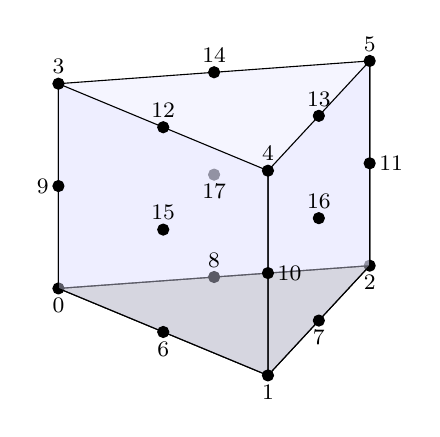
\begin{tikzpicture}[join=round]
        \filldraw[fill=black!20](1.748,.561)--(-2.205,.272)--(.456,-.833)--cycle;
        \filldraw(1.748,.561) circle (2pt);
        \filldraw(-.228,1.717) circle (2pt);
        \filldraw[fill=blue!10,fill opacity=0.4](-2.205,2.872)--(-2.205,.272)--(1.748,.561)--(1.748,3.161)--cycle;
        \filldraw[fill=blue!10,fill opacity=0.4](1.748,3.161)--(1.748,.561)--(.456,-.833)--(.456,1.767)--cycle;
        \filldraw(-.228,.417) circle (2pt);
        \filldraw(1.748,1.861) circle (2pt);
        \filldraw(-2.205,.272) circle (2pt);
        \filldraw[fill=blue!10,fill opacity=0.4](.456,1.767)--(.456,-.833)--(-2.205,.272)--(-2.205,2.872)--cycle;
        \filldraw(1.748,3.161) circle (2pt);
        \filldraw(-2.205,1.572) circle (2pt);
        \filldraw(-.228,3.017) circle (2pt);
        \filldraw(-2.205,2.872) circle (2pt);
        \filldraw(1.102,-.136) circle (2pt);
        \filldraw(-.874,-.281) circle (2pt);
        \filldraw(1.102,1.164) circle (2pt);
        \filldraw(-.874,1.019) circle (2pt);
        \filldraw(1.102,2.464) circle (2pt);
        \filldraw(-.874,2.319) circle (2pt);
        \filldraw(.456,-.833) circle (2pt);
        \filldraw(.456,.467) circle (2pt);
        \filldraw(.456,1.767) circle (2pt);
        \fill[black,font=\footnotesize]
                (-2.205,.272) node [below] {0}
                (.456,-.833) node [below] {1}
                (1.748,.561) node [below] {2}
                (-2.205,2.872) node [above] {3}
                (.456,1.767) node [above] {4}
                (1.748,3.161) node [above] {5}
                (-.874,-.281) node [below] {6}
                (1.102,-.136) node [below] {7}
                (-.228,.417) node [above] {8}
                (-2.205,1.572) node [left] {9}
                (.456,.467) node [right] {10}
                (1.748,1.861) node [right] {11}
                (-.874,2.319) node [above] {12}
                (1.102,2.464) node [above] {13}
                (-.228,3.017) node [above] {14}
                (-.874,1.019) node [above] {15}
                (1.102,1.164) node [above] {16}
                (-.228,1.717) node [below] {17};
    \end{tikzpicture}
  \end{center}
  \begin{center}(c)\end{center}
  \caption{(a) Base wedge {\tt (Wedge<>)}, (b) fifteen-node extended wedge {\tt (Wedge<15>)}, and (c) eighteen-node extended wedge {\tt (Wedge<18>)} topology in Shards.}
 \label{fig:wed1}
\end{figure}

\begin{figure}[ht]
  \begin{center}
   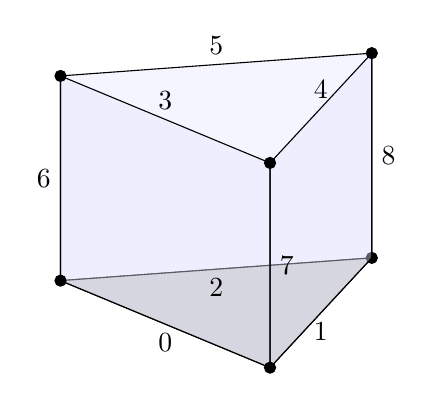
\begin{tikzpicture}[join=round] % Wedge edge numbering
       \filldraw[fill=blue!10,fill opacity=0.4](-2.205,2.872)--(-2.205,.272)--(1.748,.561)--(1.748,3.161)--cycle;
       \filldraw[fill=black!20](1.748,.561)--(-2.205,.272)--(.456,-.833)--cycle;
        \filldraw(1.748,.561) circle (2pt);
       \filldraw[fill=blue!10,fill opacity=0.4](1.748,3.161)--(1.748,.561)--(.456,-.833)--(.456,1.767)--cycle;
       \filldraw[fill=blue!10,fill opacity=0.4](.456,1.767)--(.456,-.833)--(-2.205,.272)--(-2.205,2.872)--cycle;
        \filldraw(-2.205,.272) circle (2pt);
        \filldraw(1.748,3.161) circle (2pt);
        \filldraw(-2.205,2.872) circle (2pt);
        \filldraw(.456,-.833) circle (2pt);
        \filldraw(.456,1.767) circle (2pt);
       \fill[black]
                (-.874,-.281) node [below] {0}
                (1.102,-.136) node [below] {1}
                (-.228,.417) node [below] {2}
                (-.874,2.319) node [above] {3}
                (1.102,2.464) node [above] {4}
                (-.228,3.017) node [above] {5}
                (-2.205,1.572) node [left] {6}
                (.456,.467) node [right] {7}
                (1.748,1.861) node [right] {8};
    \end{tikzpicture}
 \end{center}
 \caption{Wedge edge (1-cell) numbering in Shards.}
 \label{fig:wed2}
\end{figure}

\begin{figure}[ht]
  \begin{center}
    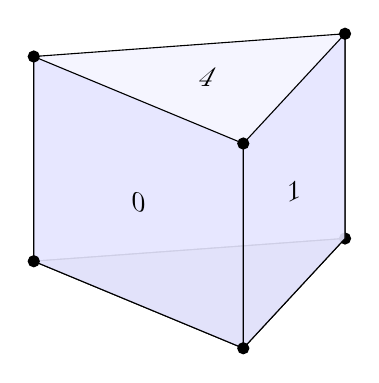
\begin{tikzpicture}[join=round] % Wedge face numbering
        \filldraw[fill=blue!10,fill opacity=0.4](-2.205,2.872)--(-2.205,.272)--(1.748,.561)--(1.748,3.161)--cycle;
        \filldraw[fill=black!20](1.748,.561)--(-2.205,.272)--(.456,-.833)--cycle;
        \filldraw(1.748,.561) circle (2pt);
        \filldraw[fill=blue!10,fill opacity=0.9](1.748,3.161)--(1.748,.561)--(.456,-.833)--(.456,1.767)--cycle;
        \filldraw[fill=blue!10,fill opacity=0.9](.456,1.767)--(.456,-.833)--(-2.205,.272)--(-2.205,2.872)--cycle;
        \filldraw(-2.205,.272) circle (2pt);
        \filldraw(1.748,3.161) circle (2pt);
        \filldraw(-2.205,2.872) circle (2pt);
        \filldraw(.456,-.833) circle (2pt);
        \filldraw(.456,1.767) circle (2pt);
        \fill[black]
                (-.874,1.019) node [yslant=-.4] {0}
                (1.102,1.164) node [yslant=.5,xslant=.0] {1}
                (0,2.6) node [xslant=.5,yslant=.0] {4};
     \end{tikzpicture}
   \hspace{1cm}
    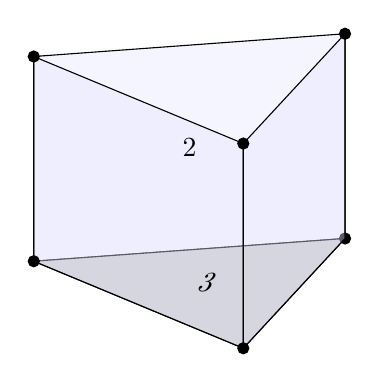
\begin{tikzpicture}[join=round] % Wedge face numbering
        \filldraw[fill=blue!10,fill opacity=0.4](-2.205,2.872)--(-2.205,.272)--(1.748,.561)--(1.748,3.161)--cycle;
        \filldraw[fill=black!20](1.748,.561)--(-2.205,.272)--(.456,-.833)--cycle;
        \filldraw(1.748,.561) circle (2pt);
        \filldraw[fill=blue!10,fill opacity=0.4](1.748,3.161)--(1.748,.561)--(.456,-.833)--(.456,1.767)--cycle;
        \filldraw[fill=blue!10,fill opacity=0.4](.456,1.767)--(.456,-.833)--(-2.205,.272)--(-2.205,2.872)--cycle;
        \filldraw(-2.205,.272) circle (2pt);
        \filldraw(1.748,3.161) circle (2pt);
        \filldraw(-2.205,2.872) circle (2pt);
        \filldraw(.456,-.833) circle (2pt);
        \filldraw(.456,1.767) circle (2pt);
        \fill[black]
                (-.228,1.717) node [] {2}
                (0,0) node[xslant=.5] {3};
     \end{tikzpicture}
 \end{center}
  \caption{Wedge face (2-cell) numbering in Shards.}
 \label{fig:wed3}
\end{figure}


\subsection{Hexahedron}
A hexahedron is an object of dimension three with eight vertices, twelve edges, and six sides. The base and extended topologies available in Shards are shown in Figure \ref{fig:hex1}. The edge numbering is shown in Figure \ref{fig:hex2} and the face numbering in Figure \ref{fig:hex3}.

 % Hexahedron node numbering
\begin{figure}[ht]
  \begin{center}
    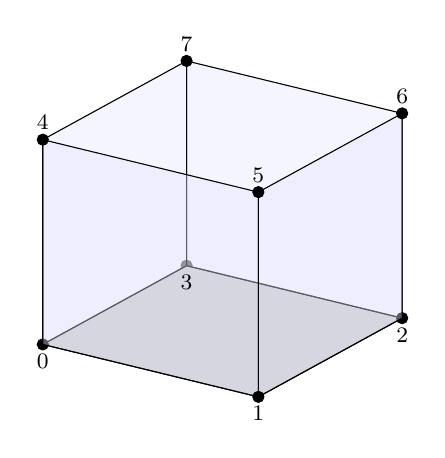
\begin{tikzpicture}[join=round] % Hex with 8 nodes
        \filldraw(-.456,.833) circle (2pt);
        \filldraw[fill=black!20](2.282,.167)--(-.456,.833)--(-2.282,-.167)--(.456,-.833)--cycle;
        \filldraw[fill=blue!10,fill opacity=0.4](-2.282,2.433)--(-2.282,-.167)--(-.456,.833)--(-.456,3.433)--cycle;
        \filldraw[fill=blue!10,fill opacity=0.4](-.456,3.433)--(-.456,.833)--(2.282,.167)--(2.282,2.767)--cycle;
        \filldraw(-.456,3.433) circle (2pt);
        \filldraw(2.282,.167) circle (2pt);
        \filldraw[fill=blue!10,fill opacity=0.4](2.282,2.767)--(2.282,.167)--(.456,-.833)--(.456,1.767)--cycle;
        \filldraw(-2.282,-.167) circle (2pt);
        \filldraw[fill=blue!10,fill opacity=0.4](.456,1.767)--(.456,-.833)--(-2.282,-.167)--(-2.282,2.433)--cycle;
        \filldraw(2.282,2.767) circle (2pt);
        \filldraw(-2.282,2.433) circle (2pt);
        \filldraw(.456,-.833) circle (2pt);
        \filldraw(.456,1.767) circle (2pt);
        \fill[black,font=\footnotesize]
                (-2.282,-.167) node [below] {0}
                (.456,-.833) node [below] {1}
                (2.282,.167) node [below] {2}
                (-.456,.833) node [below] {3}
                (-2.282,2.433) node [above] {4}
                (.456,1.767) node [above] {5}
                (2.282,2.767) node [above] {6}
                (-.456,3.433) node [above] {7};
     \end{tikzpicture}
     \hspace{1cm}
    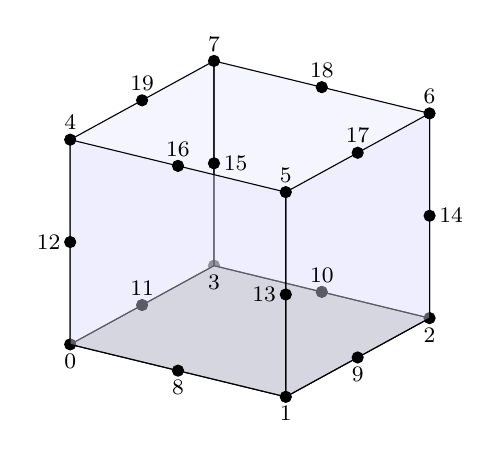
\begin{tikzpicture}[join=round] % Hex with 20 nodes
        \filldraw(-.456,.833) circle (2pt);
        \filldraw[fill=black!20](2.282,.167)--(-.456,.833)--(-2.282,-.167)--(.456,-.833)--cycle;
        \filldraw[fill=blue!10,fill opacity=0.4](-2.282,2.433)--(-2.282,-.167)--(-.456,.833)--(-.456,3.433)--cycle;
        \filldraw[fill=blue!10,fill opacity=0.4](-.456,3.433)--(-.456,.833)--(2.282,.167)--(2.282,2.767)--cycle;
        \filldraw(-.456,2.133) circle (2pt);
        \filldraw(.913,.5) circle (2pt);
        \filldraw(-.456,3.433) circle (2pt);
        \filldraw(-1.369,.333) circle (2pt);
        \filldraw(2.282,.167) circle (2pt);
        \filldraw[fill=blue!10,fill opacity=0.4](2.282,2.767)--(2.282,.167)--(.456,-.833)--(.456,1.767)--cycle;
        \filldraw(.913,3.1) circle (2pt);
        \filldraw(2.282,1.467) circle (2pt);
        \filldraw(-1.369,2.933) circle (2pt);
        \filldraw(-2.282,-.167) circle (2pt);
        \filldraw[fill=blue!10,fill opacity=0.4](.456,1.767)--(.456,-.833)--(-2.282,-.167)--(-2.282,2.433)--cycle;
        \filldraw(2.282,2.767) circle (2pt);
        \filldraw(1.369,-.333) circle (2pt);
        \filldraw(-2.282,1.133) circle (2pt);
        \filldraw(-.913,-.5) circle (2pt);
        \filldraw(-2.282,2.433) circle (2pt);
        \filldraw(1.369,2.267) circle (2pt);
        \filldraw(.456,-.833) circle (2pt);
        \filldraw(-.913,2.1) circle (2pt);
        \filldraw(.456,.467) circle (2pt);
        \filldraw(.456,1.767) circle (2pt);
        \fill[black,font=\footnotesize]
                (-2.282,-.167) node [below] {0}
                (.456,-.833) node [below] {1}
                (2.282,.167) node [below] {2}
                (-.456,.833) node [below] {3}
                (-2.282,2.433) node [above] {4}
                (.456,1.767) node [above] {5}
                (2.282,2.767) node [above] {6}
                (-.456,3.433) node [above] {7}
                (-.913,-.5) node [below] {8}
                (1.369,-.333) node [below] {9}
                (.913,.5) node [above] {10}
                (-1.369,.333) node [above] {11}
                (-2.282,1.133) node [left] {12}
                (.456,.467) node [left] {13}
                (2.282,1.467) node [right] {14}
                (-.456,2.133) node [right] {15}
                (-.913,2.1) node [above] {16}
                (1.369,2.267) node [above] {17}
                (.913,3.1) node [above] {18}
                (-1.369,2.933) node [above] {19};
    \end{tikzpicture}
  \end{center}
  \begin{center} {(a) \hspace{5cm} (b)} \end{center}
   \begin{center}
      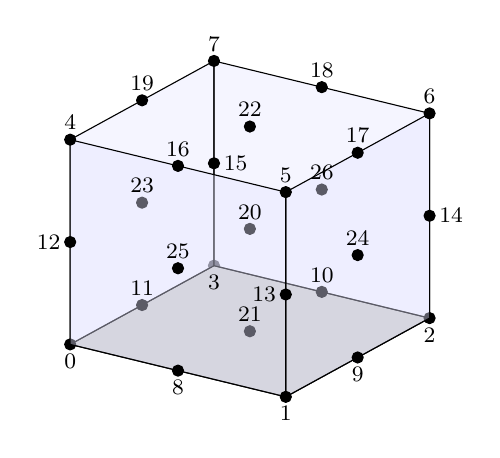
\begin{tikzpicture}[join=round]
          \filldraw(-.456,.833) circle (2pt);
          \filldraw[fill=black!20](2.282,.167)--(-.456,.833)--(-2.282,-.167)--(.456,-.833)--cycle;
          \filldraw[fill=blue!10,fill opacity=0.4](-2.282,2.433)--(-2.282,-.167)--(-.456,.833)--(-.456,3.433)--cycle;
          \filldraw[fill=blue!10,fill opacity=0.4](-.456,3.433)--(-.456,.833)--(2.282,.167)--(2.282,2.767)--cycle;
          \filldraw(-.456,2.133) circle (2pt);
          \filldraw(.913,.5) circle (2pt);
          \filldraw(-.456,3.433) circle (2pt);
          \filldraw(-1.369,.333) circle (2pt);
          \filldraw(.913,1.8) circle (2pt);
          \filldraw(2.282,.167) circle (2pt);
          \filldraw[fill=blue!10,fill opacity=0.4](2.282,2.767)--(2.282,.167)--(.456,-.833)--(.456,1.767)--cycle;
          \filldraw(-1.369,1.633) circle (2pt);
          \filldraw(.913,3.1) circle (2pt);
          \filldraw(0,0) circle (2pt);
          \filldraw(2.282,1.467) circle (2pt);
          \filldraw(-1.369,2.933) circle (2pt);
          \filldraw(-2.282,-.167) circle (2pt);
          \filldraw(0,1.3) circle (2pt);
          \filldraw[fill=blue!10,fill opacity=0.4](.456,1.767)--(.456,-.833)--(-2.282,-.167)--(-2.282,2.433)--cycle;
          \filldraw(2.282,2.767) circle (2pt);
          \filldraw(1.369,-.333) circle (2pt);
          \filldraw(-2.282,1.133) circle (2pt);
          \filldraw(0,2.6) circle (2pt);
          \filldraw(-.913,-.5) circle (2pt);
          \filldraw(1.369,.967) circle (2pt);
          \filldraw(-2.282,2.433) circle (2pt);
          \filldraw(-.913,.8) circle (2pt);
          \filldraw(1.369,2.267) circle (2pt);
          \filldraw(.456,-.833) circle (2pt);
          \filldraw(-.913,2.1) circle (2pt);
          \filldraw(.456,.467) circle (2pt);
          \filldraw(.456,1.767) circle (2pt);
          \fill[black,font=\footnotesize]
                (-2.282,-.167) node [below] {0}
                (.456,-.833) node [below] {1}
                (2.282,.167) node [below] {2}
                (-.456,.833) node [below] {3}
                (-2.282,2.433) node [above] {4}
                (.456,1.767) node [above] {5}
                (2.282,2.767) node [above] {6}
                (-.456,3.433) node [above] {7}
                (-.913,-.5) node [below] {8}
                (1.369,-.333) node [below] {9}
                (.913,.5) node [above] {10}
                (-1.369,.333) node [above] {11}
                (-2.282,1.133) node [left] {12}
                (.456,.467) node [left] {13}
                (2.282,1.467) node [right] {14}
                (-.456,2.133) node [right] {15}
                (-.913,2.1) node [above] {16}
                (1.369,2.267) node [above] {17}
                (.913,3.1) node [above] {18}
                (-1.369,2.933) node [above] {19}
                (0,1.3) node [above] {20}
                (0,0) node [above] {21}
                (0,2.6) node [above] {22}
                (-1.369,1.633) node [above] {23}
                (1.369,.967) node [above] {24}
                (-.913,.8) node [above] {25}
                (.913,1.8) node [above] {26};
    \end{tikzpicture}
  \end{center}
  \begin{center}(c)\end{center} 
 \caption{(a) Base hexahedron{\tt (Hexahedron<>)}, (b) fifteen-node extended hexahedron {\tt (Hexahedron<15>)}, and (c) eighteen-node extended hexahedron {\tt (Hexahedron<18>)} topology in Shards.}
 \label{fig:hex1}
\end{figure}

\begin{figure}[ht]
   \begin{center}
     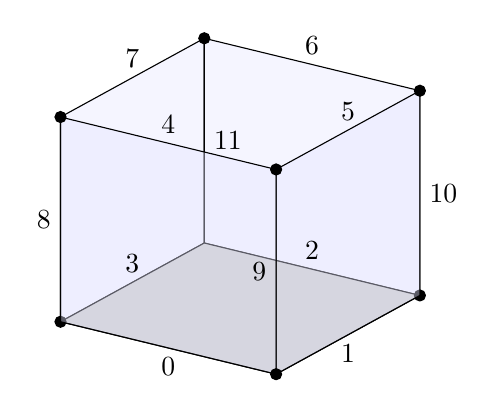
\begin{tikzpicture}[join=round] % Hexahedron Edges
         \filldraw[fill=blue!10,fill opacity=0.4](-2.282,2.433)--(-2.282,-.167)--(-.456,.833)--(-.456,3.433)--cycle;
         \filldraw[fill=blue!10,fill opacity=0.4](-.456,3.433)--(-.456,.833)--(2.282,.167)--(2.282,2.767)--cycle;
         \filldraw[fill=black!20](2.282,.167)--(-.456,.833)--(-2.282,-.167)--(.456,-.833)--cycle;
        \filldraw(-.456,3.433) circle (2pt);
        \filldraw(2.282,.167) circle (2pt);
         \filldraw[fill=blue!10,fill opacity=0.4](2.282,2.767)--(2.282,.167)--(.456,-.833)--(.456,1.767)--cycle;
        \filldraw(-2.282,-.167) circle (2pt);
         \filldraw[fill=blue!10,fill opacity=0.4](.456,1.767)--(.456,-.833)--(-2.282,-.167)--(-2.282,2.433)--cycle;
        \filldraw(2.282,2.767) circle (2pt);
        \filldraw(-2.282,2.433) circle (2pt);
        \filldraw(.456,-.833) circle (2pt);
        \filldraw(.456,1.767) circle (2pt);
         \fill[black]
                (-.913,-.5) node [below] {0}
                (1.369,-.333) node [below] {1}
                (.913,.5) node [above] {2}
                (-1.369,.333) node [above] {3}
                (-2.282,1.133) node [left] {8}
                (.456,.467) node [left] {9}
                (2.282,1.467) node [right] {10}
                (-.456,2.133) node [right] {11}
                (-.913,2.1) node [above] {4}
                (1.369,2.267) node [above] {5}
                (.913,3.1) node [above] {6}
                (-1.369,2.933) node [above] {7};
     \end{tikzpicture}
  \end{center}
 \caption{Hexahedron edge (1-cell) numbering in Shards.}
 \label{fig:hex2}
\end{figure}

\begin{figure}[ht]
  \begin{center}
     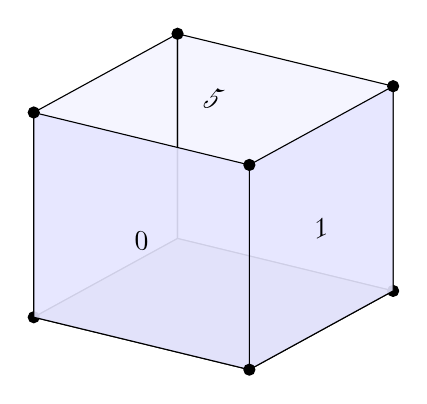
\begin{tikzpicture}[join=round] % Hexahedron Faces
         \filldraw[fill=blue!10,fill opacity=0.4](-2.282,2.433)--(-2.282,-.167)--(-.456,.833)--(-.456,3.433)--cycle;
         \filldraw[fill=blue!10,fill opacity=0.4](-.456,3.433)--(-.456,.833)--(2.282,.167)--(2.282,2.767)--cycle;
         \filldraw[fill=black!20](2.282,.167)--(-.456,.833)--(-2.282,-.167)--(.456,-.833)--cycle;
         \filldraw(-.456,3.433) circle (2pt);
         \filldraw(2.282,.167) circle (2pt);
         \filldraw[fill=blue!10,fill opacity=0.9](2.282,2.767)--(2.282,.167)--(.456,-.833)--(.456,1.767)--cycle;
         \filldraw(-2.282,-.167) circle (2pt);
         \filldraw[fill=blue!10,fill opacity=0.9](.456,1.767)--(.456,-.833)--(-2.282,-.167)--(-2.282,2.433)--cycle;
         \filldraw(2.282,2.767) circle (2pt);
         \filldraw(-2.282,2.433) circle (2pt);
         \filldraw(.456,-.833) circle (2pt);
         \filldraw(.456,1.767) circle (2pt);
         \fill[black]
                (0,2.6) node [xslant=.8,yslant=-.2] {5}
                (1.369,.967) node [yslant=0.5] {1}
                (-.913,.8) node [yslant=-.2] {0};
      \end{tikzpicture}
     \hspace{1cm}
     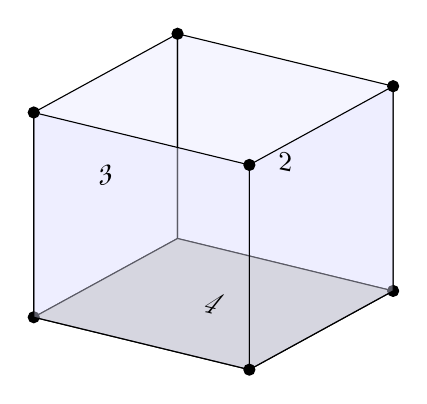
\begin{tikzpicture}[join=round] % Hexahedron Faces
         \filldraw[fill=blue!10,fill opacity=0.4](-2.282,2.433)--(-2.282,-.167)--(-.456,.833)--(-.456,3.433)--cycle;
         \filldraw[fill=blue!10,fill opacity=0.4](-.456,3.433)--(-.456,.833)--(2.282,.167)--(2.282,2.767)--cycle;
         \filldraw[fill=black!20](2.282,.167)--(-.456,.833)--(-2.282,-.167)--(.456,-.833)--cycle;
         \filldraw(-.456,3.433) circle (2pt);
         \filldraw(2.282,.167) circle (2pt);
         \filldraw[fill=blue!10,fill opacity=0.4](2.282,2.767)--(2.282,.167)--(.456,-.833)--(.456,1.767)--cycle;
         \filldraw(-2.282,-.167) circle (2pt);
         \filldraw[fill=blue!10,fill opacity=0.4](.456,1.767)--(.456,-.833)--(-2.282,-.167)--(-2.282,2.433)--cycle;
         \filldraw(2.282,2.767) circle (2pt);
         \filldraw(-2.282,2.433) circle (2pt);
         \filldraw(.456,-.833) circle (2pt);
         \filldraw(.456,1.767) circle (2pt);
         \fill[black]
                (0,0) node [xslant=0.8,yslant=-.2] {4}
                (-1.369,1.633) node [yslant=0.5] {3}
                (.913,1.8) node [yslant=-.2] {2};
      \end{tikzpicture}
  \end{center}
 \caption{Hexahedron face (2-cell) numbering in Shards.}
 \label{fig:hex3}
\end{figure}

    % \printindex

    \begin{SANDdistribution}[NM]% or [CA]
	% \SANDdistCRADA	% If this report is about CRADA work
	% \SANDdistPatent	% If this report has a Patent Caution or Patent Interest
	% \SANDdistLDRD	% If this report is about LDRD work

	% External Address Format: {num copies}{Address}
        \SANDdistExternal{1}{}
	\bigskip

	% The following MUST BE between the external and internal distributions!
	% \SANDdistClassified % If this report is classified
        \SANDdistInternal{1}{1320}{Kenneth Alvin}{1414}
        \SANDdistInternal{1}{1318}{Roscoe Bartlett}{1411}
        \SANDdistInternal{2}{1320}{Pavel Bochev}{1414}
        \SANDdistInternal{1}{1320}{Scott Collis}{1414}
        \SANDdistInternal{2}{1541}{Harold Edwards}{1541}
        \SANDdistInternal{1}{0316}{Rob Hoekstra}{1437}
        \SANDdistInternal{1}{1318}{Roger Pawlowski}{1416}
        \SANDdistInternal{1}{1318}{Eric Phipps}{1416}
        \SANDdistInternal{2}{1318}{Denis Ridzal}{1411}
        \SANDdistInternal{1}{1320}{Andrew Salinger}{1414}
        \SANDdistInternal{1}{0316}{John Shadid}{1437}
        \SANDdistInternal{1}{1318}{Bart van Bloemen Waanders}{1411}
        \SANDdistInternal{2}{0612}{Review \& Approval Desk}{4916}
	% Internal Address Format: {num copies}{Mail stop}{Name}{Org}

	% Mail Channel Address Format: {num copies}{Mail Channel}{Name}{Org}
	%\SANDdistInternalM{}{}{}{}
    \end{SANDdistribution}


    % The second printing
    %\begin{SANDreDistribution}
    %    \SANDdistExternal{}{}
    %    \bigskip
    %    \SANDdistInternal{}{}{}{}
    %    \SANDdistInternalM{}{}{}{}
    %\end{SANDreDistribution}
\end{document}
